\documentclass{article}

%%%%%%%%%%%%%%%%%%%%%%%%%%%%%%%%%%%%%%%%%%%%%%%%%%%%%%%%%%%%%%%%%%%%%%%%%%%%%%%%
%% package setup
%%%%%%%%%%%%%%%%%%%%%%%%%%%%%%%%%%%%%%%%%%%%%%%%%%%%%%%%%%%%%%%%%%%%%%%%%%%%%%%%

\usepackage{enumerate}
\usepackage[shortlabels]{enumitem}
\usepackage{amsfonts,amsmath, soul, matlab-prettifier, bm, amsthm,enumitem,amssymb,multirow,float,mathtools,bbm,array,varwidth,hyperref, etoolbox}
\usepackage[all]{xy}
\usepackage[margin=0.9in]{geometry}
\usepackage{graphicx}
\usepackage{mathtools}
\usepackage{extarrows}
\usepackage{tikz}
\usepackage{tikz-cd}
%\usepackage{bbold}
\usepackage[OT2,T1]{fontenc}
\usepackage{calrsfs}
\usepackage{dsfont}
\usepackage[title]{appendix}
\usepackage{wrapfig}
\usepackage{subcaption}

\raggedbottom

%%%%%%%%%%%%%%%%%%%%%%%%%%%%%%%%%%%%%%%%%%%%%%%%%%%%%%%%%%%%%%%%%%%%%%%%%%%%%%%%
%% operators and symbols
%%%%%%%%%%%%%%%%%%%%%%%%%%%%%%%%%%%%%%%%%%%%%%%%%%%%%%%%%%%%%%%%%%%%%%%%%%%%%%%%

\newcommand{\define}[4]{\expandafter#1\csname#3#4\endcsname{#2{#4}}}

% operators
\forcsvlist{\define{\DeclareMathOperator}{\mathrm}{}}{Ad, Aut, BSD, Char, Cl, Det, End, Frob, Gal, GL, hol, Hom, Id, Ind, Irr, Jac, Ker, Mod, new, old, ord,  Perm, PGL, Pic, Proj, PSL, Rad, Reg, Rep, res, Res, rk, sign, SL, Smo, SO, Span, Spec, Stab, supp, sw, Sym, Ta, tors, Tr, Trace, un, Vect, contr, Sel, rad, Norm}

%trivial and ell
\newcommand{\trivial}{\mathbbm{1}}
%\renewcommand{\ell}{l}

%mathbb letters 
\forcsvlist{\define{\newcommand}{\mathbb}{b}}{1,A,B,C,D,E,F,G,H,I,J,K,L,M,N,O,P,Q,R,S,T,U,V,W,X,Y,Z}

%mathcal letters
\forcsvlist{\define{\newcommand}{\mathcal}{c}}{A,B,C,D,E,F,G,H,I,J,K,L,M,N,O,P,Q,R,S,T,U,V,W,X,Y,Z,a,v}

%mathfrak letters
\forcsvlist{\define{\newcommand}{\mathfrak}{f}}{A,B,C,D,E,F,G,H,I,J,K,L,M,N,O,P,Q,R,S,T,U,V,W,X,Y,Z,a,m,n,p,q, g, t}

%overline letters
\forcsvlist{\define{\newcommand}{\overline}{ov}}{H,I,J,K,L,M,N,O,P,Q,R,S,T,U,V,W,X,Y,Z,a,b,c,d,e,f,g,h,i,j,k,l,m,n,o,p,q,r,s,t,u,v,w,x,y,z}

% mathbb
\newcommand{\CC}{\mathbb{C}}
\newcommand{\FF}{\mathbb{F}}
\newcommand{\NN}{\mathbb{N}}
\newcommand{\PP}{\mathbb{P}}
\newcommand{\QQ}{\mathbb{Q}}
\newcommand{\RR}{\mathbb{R}}
\newcommand{\ZZ}{\mathbb{Z}}
\newcommand{\GG}{\mathbb{G}}
\newcommand{\adele}{\mathbb{A}}
\newcommand{\pp}{\mathfrak{p}}
\newcommand{\qq}{\mathfrak{q}}
\newcommand{\rr}{\mathfrak{r}}

% mathfra
%\newcommand{\fg}{\mathfrak{g}}
%\newcommand{\fm}{\mathfrak{m}}

\newcommand{\norm}[1]{\left\lVert#1\right\rVert}
\newcommand{\hatv}[1]{\overset{\vee}{\mathstrut#1}}

% Structures
\def\set#1{\left\{#1\right\}}
%\def\sets#1#2{\left\{\left.#1\ \right\vert#2\right\}}
\def\rbr#1{\left(#1\right)}
\def\ang#1{\left\langle#1\right\rangle}
\def\n#1{\left\lvert#1\right\rvert}
\def\nn#1{\left\lVert#1\right\rVert}
\def\eq#1{\begin{equation}#1\end{equation}}
\def\ov#1#2{{\substack{#1\\#2}}} % #1 over #2

% Symbols
\def\mto{\mapsto}
\def\emb{\hookrightarrow}
\def\es{\emptyset}
\def\bs{\backslash}
\def\cupp{\smallsmile}
\def\surj{\twoheadrightarrow}

% floor and ceiling
\DeclarePairedDelimiter\ceil{\lceil}{\rceil}
\DeclarePairedDelimiter\floor{\lfloor}{\rfloor}

\DeclareMathOperator{\Ima}{Im}
\linespread{1.5}

\theoremstyle{plain}
\newtheorem{thm}{Theorem}[section]
\newtheorem{question}[thm]{Question}
\newtheorem{prop}[thm]{Proposition}
\newtheorem{condition}[thm]{Condition}
\newtheorem{lemma}[thm]{Lemma}
\newtheorem{cor}[thm]{Corollary}
\newtheorem{algo}[thm]{Algorithm}
\theoremstyle{definition}
\newtheorem{defn}[thm]{Definition}
\newtheorem{notn}[thm]{Notation}
\newtheorem{rem}[thm]{Remark}
\newtheorem{example}[thm]{Example}
\newtheorem{examples}[thm]{Examples}
\newtheorem{fact}[thm]{Fact}

\newtheorem{conj}[thm]{Conjecture}
\newtheorem{notation}[thm]{Notation}

%Sha:
\usepackage[OT2,T1]{fontenc}
\DeclareSymbolFont{cyrletters}{OT2}{wncyr}{m}{n}
\DeclareMathSymbol{\Sha}{\mathalpha}{cyrletters}{"58}
%end of Sha

%\DeclareSymbolFont{cyrletters}{OT2}{wncyr}{m}{n}
%\DeclareMathSymbol{\Sha}{\mathalpha}{cyrletters}{"58}

%\DeclareMathAlphabet{\pazocal}{OMS}{zplm}{m}{n}


\title{Arithmetic Applications of Artin Twist and BSD}
\author{Edwina Aylward, Albert Lopez Bruch}

\begin{document}
	\maketitle
	\pagenumbering{arabic}
	\newpage
	\tableofcontents
	\newpage

\section*{Introduction}
In this report we study a method proposed in \cite{DEW1} for forcing points of infinite order on elliptic curves over finite extensions $F / \bQ$. 

\subsection*{Notation}
We use the following notation for characters:

\bigskip

\begin{tabular}{l | l}
    $R_(G)$ & the representation ring of $G$, \\
    $R_{\bQ}(G)$ & the rational representation ring of $G$, \\
    $\Perm(G)$ & the ring of virtual permutations of $G$, \\
    $\Char_{\bQ}(G)$ & the ring of rationally-valued characters of $G$,\\
    $\Irr(G)$ & the set of characters of complex irreducible representations of $G$, \\
    %$\Irr_{\bQ}(G)$ & the set of characters of $\bQ$-irreducible representations of $G$, \\ 
    $\bQ(\rho)$ & the field of character values of a complex character $\rho$ of $G$, \\
    $C(G)$ & the finite abelian group $\Char_{\bQ}(G) / \Perm(G)$, \\ 
    %$m(\rho)$ & the Schur Index of an irreducible complex character $\rho$ over $\bQ(\rho)$, \\
    \\
    $H^{x}$ & $= xHx^{-1}$  for $H \leq G$ a subgroup of a group $G$ and $x \in G$,
\end{tabular}
\vspace{2em}

Given an elliptic curve $E / \bQ$ and a number field $F$, we define

\[ C_{E / F} = \prod_v c_v(E / F) \left| \frac{\omega}{\omega_v^{\min}} \right|_v. \]
The product is taken over the finite places of $F$, $\omega$ is a global minimal differential for $E / \bQ$, and $\omega_v^{\min}$ is a minimal differential at $v$. In terms of minimal discriminants, if $E$ is of the form
\[ y^2 + a_1 x y + a_3 y = x^3 + a_2 x^2 + a_4 x + a_6 \]
with minimal discriminant $\Delta_E$ and $\omega = \frac{dx}{2 y + a_1 x + a_3}$, then
\[ \left| \frac{\omega}{\omega_v^{\min}} \right|_v^{-12} = \left| \frac{\Delta_E}{\Delta_{E, v}^{\min}} \right|_v . \]

\newpage
\section{Norm relations}
\subsection{Representations of finite groups}\label{rep}

Let $G$ be a finite group, $K$ a field of characteristic zero. Recall that a \textbf{representation} of $G$ over $K$ is a group homomorphism $\rho \colon G \to \GL(V)$ where $V$ is a $K$-vector space. Associated to a representation $\rho$ is a \textbf{character} $\chi \colon G \to K^{\times}$, defined by letting $\chi(g) = \Tr \rho(g)$ for $g \in G$. For complex representations, $\rho$ is determined by its character; if $\rho$, $\rho'$ are representations with identical characters, then $\rho$ and $\rho'$ are isomorphic as representations. 

\begin{defn}
Let $\chi_1, \ldots \chi_h$ be the distinct characters of the complex irreducible representations of $G$. 
Then the \textbf{representation ring} of $G$ is 
\[ R(G) = \bZ \chi_1 \oplus \cdots \oplus \bZ \chi_h .\]
%We can also view this as the Grothendieck group of the category of finitely generated $\bC[G]$-modules.
\end{defn}

Since we take differences of characters in $R(G)$, we sometimes call elements of $R(G)$ \textbf{virtual representations}. 

Let $K$ be a number field. Denote by $R_K(G)$ the group generated by characters of the representations of $G$ over $K$. This is a subring of $R(G)$.
When $K = \bQ$ this is called the \textbf{rational representation ring}.
The characters of the distinct irreducible representations of $G$ over $K$ form an orthogonal basis of $R_K(G)$ (\cite[Proposition 32]{Serre}).
Let $m$ be the exponent of $G$. If $K$ contains the $m$-th roots of unity, then $R_K(G) = R(G)$ (\cite[Theorem 24]{Serre}). This implies every representation of $G$ can be realized over such $K$. 
\vspace{1em}

%The rank of $R_K(G)$ is discussed in {\color{red} Serre 12.4}.
Let $\Perm(G)$ be the ring of virtual permutation representations of $G$ (i.e. the ring generated by the characters of $\bC[G / H]$ for $H \leq G$). Let $\Char_{\bQ}(G)$ be the ring of rationally valued characters of $G$. Then we have inclusions 
\[ \Perm(G) \to R_{\bQ}(G) \to \Char_{\bQ}(G). \]
Each of these groups have equal $\bZ$-rank, equal to the number of conjugacy classes of cyclic subgroups of $G$ {\color{red} ref}. Moreover the cokerenels of these maps are finite.

It is of interest to obtain characters of $\Perm(G)$ from characters of $R(G)$.
For $\rho \in R(G)$ one obtains an element of $\Char_{\bQ}(G)$ by taking 
$$ {\widetilde{\rho}} = \sum_{\sigma \in \Gal(\bQ(\rho)/\bQ)}  \rho^\sigma \quad .$$
Here $\bQ(\rho)$ means the smallest Galois field extension that contains the values of $\rho(g)$ for all $g \in G$, and $\rho^\sigma$ is the character such that $\rho^\sigma(g) = \sigma(\rho(g))$. Conversely, if a representation has a rationally valued character, then any complex irreducible constituent must occur along with all its Galois conjugates with equal multiplicity. Therefore our map $R(G) \to \Char_{\bQ}(G)$ is surjective.

Such a character may not be in $R_{\bQ}(G)$, however. That is, it has rational character, but the corresponding representation cannot be realized over $\bQ$. The quotient $\Char_{\bQ}(G) / R_{\bQ}(G)$ is the study of Schur indices.  If $\rho \in R(G)$ is an irreducible representation, the \textbf{Schur index} is the smallest integer $m(\rho)$ such that 
\[ \sum_{\sigma \in \Gal(\bQ(\rho)/\bQ)}m(\rho) \cdot \rho^\sigma \quad \in R_{\bQ}(G). \]

We are more interested in the group $$C(G) = \Char_{\bQ}(G) / \Perm(G).$$ This is a finite abelian group. It has exponent dividing $|G|$ by Artin's induction theorem {\color{red} ref}. The study of this group is quite subtle, see for example \cite{Tim-Alex}. For us, it's enough to know that there exists an integer $m$ dividing $|G|$ such that $\widetilde{\rho}^{\ \oplus m } \in \Perm(G)$, where $m$ is the order of $\widetilde{\rho}$ in $C(G)$. Thus, we have a map $\Irr(G) \to \Perm(G)$. We extend this additively to a map $R(G) \to \Perm(G)$.

{\color{red} could add some examples of when $C(G)$ is trivial}

%\begin{notn}
%For $\rho \in R_{\bC}(G)$ an irreducible character let 
%\[  \widetilde{\rho} = \sum_{\sigma \in \Gal(\bQ(\rho)/\bQ)}m(\rho)\cdot \rho^\sigma \quad \in R_{\bQ}(G) , \]
%where $m(\rho) \in \bZ$ is the Schur index of $\rho$.
%\end{notn}
%Then $\widetilde{\rho}$ is the character of an irreducible rational representation. Every irreducible rational representation can be obtained this way. We can extend this map additively to a surjective map $R_{\bC}(G) \to R_{\bQ}(G)$. 

%Let $\overline{R_K(G)}$ be the subring of elements of $R(G)$ which have values in $K$. Then $R_K(G) \subset \overline{R_K(G)}$ and this inclusion is of finite index. 
%Given a character $\chi$ of $G$, let $\bQ(\chi)$ be the smallest subfield of $\bC$ containing $\{ \chi(g) \mid g \in G \}$.
%Let $R_{\bC}(G)$ denote the ring of characters of complex representations of $G$. The number of complex irreducible representations of $G$ is equal to the number of conjugacy classes of $G$. Let $R_{\bQ}(G)$ be the ring of characters of rational valued representations of $G$.
%The number of irreducible $\bQ G$-representations up to isomorphism is equal to the number of conjugacy classes of cyclic subgroups of $G$. %(\cite[$\mathsection 13.1$, Cor. 1]{Serre})
%Induction, Restriction\dots
%\begin{thm}[Mackey Decomposition] 
%\end{thm} 

\subsection{The Burnside ring and \color{red} permutation relations}

Let $G$ be a finite group. Recall that there is a bijection between the isomorphism classes of transitive finite $G$-sets and the conjugacy classes of subgroups $H \leq G$, given by sending a transitive $G$-set $X$ to $H = \Stab_{G}(x)$ for some $x \in X$. Then the action of $G$ on $X$ is equivalent to the action of $G$ on $G / H$. 

\begin{defn}
Let $[X]$ denote the isomorphism class of a $G$-set $X$. 
The \textbf{Burnside ring} $B(G)$ is the free abelian group on isomorphism classes of finite $G$-sets, modulo the relations  $[S] + [T] = [S \sqcup T]$. This is a ring; multiplication is given by $[S] \cdot [T] = [S \times T]$. Using the identification of finite $G$-sets with subgroups of $G$, we write elements of $B(G)$ as $\sum_i n_i H_i$ for $n_i \in \bZ$, $H_i \leq G$. 
\end{defn}

\begin{notn}
There is a homomorphism from the Burnside ring to the rational representation ring $R_{\bQ}(G)$ of $G$ given by taking the corresponding permutation representation:
\[ \bC[-] \colon B(G) \to \Perm(G),  \qquad \Theta = \sum_i n_i H_i \ \mapsto \ \bC[\Theta ] = \sum_i n_i \Ind_{H_i}^G \trivial_{H_i}. \]
\end{notn}
Elements in the kernel of this map are known as \textbf{Brauer relations}. These show instances of non-isomorphic $G$-sets giving rise to isomorphic permutation representations. 

\begin{example}
    {\color{red} $S_3$ example}
\end{example}

\begin{example}
Cyclic groups have no Brauer relations. 
\end{example}

In the last section, we constructed a character in $\Perm(G)$ for $\rho \in R(G)$. We are interested in when this is an image of an element from the Burnside ring.

\begin{defn}
We call $\Theta = \sum_i n_i H_i \in B(G)$ a \textbf{$\rho$-relation} if $\bC[\Theta] \simeq \widetilde{\rho}^{\ \oplus m}$, where $m$ is the order of $\widetilde{\rho}$ in $C(G)$.
\end{defn}
There are $\#$(Brauer relations) $+ 1$ such elements $\Theta$ {\color{red} expand on why?}. Of course, when $\rho = 0$ these are Brauer relations. 


\begin{example}\label{cyclic-relns}
    Let $G = C_n$. For each $d \mid n$, let $\chi_d = \widetilde{\varphi_d}$, where $\varphi_d$ is an irreducible complex character of $G$ with field of values $\bQ(\zeta_d)$ and kernel of index $d$.
    Then $\{ \chi_d \colon d\mid n \}$ form an orthogonal basis for the irreducible rational-valued representations of $G$. Note that $\Ind_{C_{n/ d}}^G \trivial$ is the direct sum of irreducible complex representations of $G$ contain $C_{n / d}$ in their kernel. Thus, $\Ind_{C_{n/ d}}^G \trivial \simeq \sum_{d' \mid d} \chi_{d'}$. Applying M\"{o}bius inversion, we obtain the \textit{unique} $\varphi_d$-relation for each $d \mid n$:
    \[ \chi_d = \sum_{d' \mid d} \mu(d / d') \cdot \Ind_{C_{n/ d}}^G \trivial. \]
    \end{example}

\begin{notn}
    For $D \leq G$, define maps $\Res_D \colon B(G) \to B(D)$ and $\Ind_D \colon B(D) \to B(G)$ by
    \[  \Res_D H = \sum_{x \in H \backslash G / D} D \cap H^{x^{-1}}, \qquad \quad \Ind_D H = H. \]
    These correspond to the representation theory side, where $\Res_D \Ind_{H}^G \trivial = \sum_{x \in H \backslash G / D} \Ind_{D \cap H^{x^{-1}}}^D \trivial$ (Mackey's decomposition), and $\Ind_{D}^G\Ind_{H}^D \trivial = \Ind_{H}^G \trivial$.
\end{notn}
\subsection{Functions on the Burnside ring and norm relations}

Consider a multiplicative function $f \colon B(G) \to A$, where $A$ is an abelian group. As in \cite{reg-const}, say that $f$ is \textbf{representation theoretic} if $f$ is trivial on Brauer relations. This means that for a $G$-set $X$, $f$ only depends on the representation $\bC[X]$. 

\begin{example}
  Let $V$ be a representation of $G$. The function $\psi(H) = \dim V^H$ is trivial on Brauer relations, as $\dim V^H = \langle \Res_{H} V , \trivial_H \rangle = \langle V, \Ind_{H}^G \trivial \rangle$ by Frobenius reciprocity.
\end{example}

We want to extend this notion and consider functions that are trivial on $\rho$-relations.
Take a multiplicative function on the Burnside ring of the form $\psi \colon B(G) \to \bQ^{\times}$. Given $\rho \in R_{\bC}(G)$ we can extend such functions from the Burnside ring to $\overline{\psi} \colon B(G) \to \bQ^{\times} / N_{\bQ(\rho) / \bQ}(\bQ(\rho)^\times)$. {\color{red} try motivate this a bit better, e.g. why do we expect functions to give norms... try relate this back to introduction}

\begin{defn}
If $\Theta \in \ker \overline{\psi}$, then $\psi(\Theta)$ is the norm of an element from $\bQ(\rho)^{\times}$. We call an instance of this a \textbf{norm relation}.
\end{defn}

\begin{defn}
 We say two functions $\psi$, $\psi'$ are \textbf{$\rho$-equivalent}, written $\psi \sim_{\rho} \psi'$, if $\overline{\psi /\psi'}$ is trivial on all $\rho$-relations. Equivalently, $\psi(\Theta) / \psi'(\Theta)$ is a norm relation for all $\rho$-relations $\Theta$. 
\end{defn}

\begin{example}
    Let $G = C_p$ for $p$ a prime. Let $\rho$ be a character of degree $p$. There is a unique $\rho$-relation given by $\Theta = C_1 - C_p$. Let $\psi(H) = [G \colon H]$. Then $\psi(\Theta) = p$, which is a norm from $\bQ(\sqrt{p^*}) \subset \bQ(\zeta_p)$ by Corollary \ref{p-norm}. 
\end{example}

\begin{example}
Let $E / \bQ$ be an elliptic curve, $G = \Gal(F / \bQ)$ for $F / \bQ$ a Galois extension. For $H \leq G$, the function $\psi \colon H \mapsto C(E / F^H)$ extends to a multiplicative function on the Burnside ring. Given a representation $\rho$ of $G$, one can ask when $\psi \sim_{\rho} 1$.
\end{example}

\subsection{D-local functions}\label{D-loc}





{\color{red} Maybe just add in definition of D-local function, and explain all this way better. Maybe also some parts of Theorem 2.36 in the reg consts paper (the parts that translate).}

(This is taken from section 2.3 of Vlad and Tim's regulator constants paper.)

Consider $G = \Gal(F / \bQ)$ and intermediate field $F^H$ for $H < G$. Let $p$ be a prime with decomposition group $D$ in $G$. 
Then the primes above $p$ in $F^H$ correspond to double cosets $H\backslash G/ D$. If a prime $w$ in $F^H$ corresponds to the double coset $HxD$, then its decomposition and inertia groups in $F / F^H$ are $H \cap D^x$ and $H \cap I^x$ respectively. In particular, the ramification degree and residue degree over $\bQ$ are given by $e_w = \frac{|I|}{|H \cap I^x|}$ and $f_w = \frac{[D \colon I]}{[H \cap D^x \colon H \cap I^x]}$. 

Our fudge factors $C(E / F)$ are defined locally; one has $C(E / F) = \prod_v c_v(E / F) \cdot |\omega / \omega_{v, \min}|$. Here $v$ runs over finite places of $F$, $\omega$ is a global minimal differential for $E / \bQ$, and $\omega_{v, \min}$ is a minimal differential at $v$.
Considering the function $H \mapsto C(E / F^H)$, and writing $C_p(E / F^H) =\prod_{v | p} c_v(E / F)\cdot |\omega / \omega_{v, \min}|$ one has

\[ \sum_{i} n_i H_i \mapsto \prod_i C(E / F^{H_i})^{n_i} = \prod_{p} C_p(E / F^H)^{n_i}. \]
Therefore, our function is the product of local functions for each $p$. Since $C_p(E / F^H)$ depends on $e_w$, $f_w$ for $w | p$, we are motivated to define the following:

\begin{defn}\label{D-I-fn}
    Suppose $I \triangleleft D < G$ with $D / I$ cyclic, and $\psi(e,f)$ is a function of $e, f \in \bN$. Define
    \[ \left(D, I, \psi\right) \colon \quad H \mapsto \prod_{x \in H\backslash G / D} \psi\left(\frac{|I|}{|H \cap I^x|}, \frac{[D \colon I]}{[H \cap D^x \colon H \cap I^x]}\right). \]
    Then, this is a function on the Burnside ring.
\end{defn}

{\color{red} try make thick brackets}
\begin{example}
For semi-stable reduction, we're considering $\psi(e, f) = e$ (the Tamagawa number). For the $d_v$ terms in the case of additive potentially good reduction at p ($p$ not equal to $2$ or $3$), we consider $\psi(e, f) = p^{f \floor{e n /12}}$, where $n \in \{2,3,4,6,9,10\}$.
\end{example}

\begin{example}\label{trivial-on-brauer}
    Let $\rho = 0$. If $W$ is a group of odd order, then $(W, W, e) \sim 1$ as functions to $\bQ^{\times} / \bQ^{\times 2}$.
    More generally if $D$ has odd order and $I \triangleleft D$ then $(D, I, e) \sim_{\rho} 1$. {\color{red} explain and reference}
\end{example}




\newpage
\section{Representations, L-functions and Artin Twists}
The Birch-Swinnerton-Dyer conjecture classically provides a connection between the arithmetic of elliptic curves and their $L$-functions. In this prelimiary section, we explore the classical definition of $L$-functions attached to an elliptic curve and their twists, and we explore some of the relevant properties that we will use later on. To do so, we first need to explore the notion of an Artin representation and of an $\ell$-adic representation. 

Throughout this section we fix a field $K$, which will either be a number field or a local field of characteristic $0$. We always specify what $K$ is in each context. We also fix an algebraic closure $\hat{K}$ of $K$ and we denote by $G_K$ the absolute galois group $\Gal(\bar{K}/K)$ of $K$. We recall that $G_K$ is a profinite group
$$G_K=\varprojlim_{F}\Gal(F/K),$$
where $F$ ranges over the finite Galois extensions of $K$ and therefore has a natural topology where a basis of open sets is given by $\Gal(\bar{K}/F)$ where $F$ is a finite extension of $K$.

\subsection{Artin Representations and  \texorpdfstring{$\ell$}{TEXT}-adic Representations} \label{subsection_reps}

We begin by recalling the notion of an Artin representation.

\begin{defn}
    Let $K$ be a number field or a local field. An \textbf{Artin representation} $\rho$ over $K$ is a complex finite-dimensional vector space $V$ together with a homomorphism $\rho:G_K\to\GL(V)=\GL_n(\CC)$ such that there is some finite Galois extension $F/K$ with $\Gal(\bar{K}/F)\subseteq\ker\rho$. In other words, $\rho$ factors through $\Gal(F/K)$ for some finite extension $F$ of $K$.
\end{defn}

Hence, an Artin representation can be equivalently viewed as a finite dimensional representation of $\Gal(F/K)$ where $F$ is some finite Galois extension of $K$. Throughout the document, we will use both notions and refer to either of them as Artin representations. Which notion we refer to is always clear from context.

\begin{rem}
    The condition above that $\Gal(\bar{K}/F)\subseteq\ker\rho$ is equivalent to $\ker\rho$ being open in $G_K$. This condition is clearly equivalent to $\rho$ being continuous with respect the discrete topology on $\GL_n(\CC)$. Interestingly, the profinite topology of $G_K$ has an surprising consequence: this condition is also equivalent to continuity with respect to the usual complex topology on $\GL_n(\CC)$. 
    %Necessity is clear, and the proof of sufficiency relies on the fact that under the complex topology, `small' neighbourhoods of the identity in $\GL(V)=\GL_n(\CC)$ do not contain any non-trivial subgroups. Hence, if $\phi:G_K\to\GL(V)$ is continuous with respect to the complex topology and $U$ is such a neighbourhood in $\GL(V)$, then $\phi^{-1}(U)\subseteq\ker\phi$ and $\phi^{-1}(U)$ is open, showing that $\ker\phi$ is open too. 
    Hence, Artin representations are simply continuous group homomorphisms $\rho:G_k\to\GL_n(\CC)$.
\end{rem}

Next, we define the notion of an $\ell$-adic representation, which will be needed to define the $L$-function of an elliptic curve. This is the local analogue of an Artin representation.

\begin{defn}
    Let $K$ be a number field or a local field. A \textbf{continuous $\ell$-adic representation} $\rho$ over $K$ is a continuous homomorphism $\rho:G_K\to\GL_n(F)$ where $F$ is a finite extension of $\QQ_\ell$ and $\GL_n(F)$ is equipped with the $\ell$-adic topology.
\end{defn}

\begin{rem} \label{rem_cont_ladic}
    The topologies on $\GL_n(\CC)$ and $\GL_n(\QQ_\ell)$ are very different, and in particular and $\ell$-adic representation may not have an open kernel. Instead, continuity is equivalent to the following condition: for every $m\geq1$, there is some finite field extension $F_m$ of $K$ such that for all $g\in\Gal(\bar{K}/F_m)$, $\rho(g)\equiv \mathrm{Id}_n\pmod{\ell^m}$.
\end{rem}

Given an Artin representation $\rho$, one can view it as homomorphism $\rho:G_K\to\GL_n(\bar{\QQ})$ and since it factors through a finite quotient, we can realise it as $\rho:G_K\to\GL_n(F)$ for some number field $F$. Hence, if $\ell$ is any rational prime and $\mathfrak{l}$ is a prime in $F$ above $\ell$, then one can realise $\rho$ as an $\ell$-adic representation $$\rho:G_K\longrightarrow\GL_n(F_\mathfrak{l}),$$
which is continuous since $\rho$ factors through a finite quotient. Furthermore, Artin and $\ell$-adic representations over $K$ have more structure; namely, one can take \textbf{direct sums} and \textbf{tensor products} in the natural way.

%We describe the construction for Artin representations, since the $\ell$-adic case is completely analogous. Suppose we have two Artin representations $\rho_1,\rho_2$ over $K$, and by the discussion on the preceding paragraph we can realise them as maps $\rho_i:G_K\to\GL_{n_i}(L_i),\ i=1,2$ where $L_1$ and $L_2$ are number fields. If we let $L=L_1L_2$, then the natural maps $\rho_1\oplus\rho_2:G_K\to\GL_{n_1+n_2}(L)$ and $\rho_1\otimes\rho_2:G_K\to\GL_{n_1n_2}(L)$ are both Artin representations. One can also show that this construction is also well-defined up to equivalence.

Finally, we discuss the notion of an induced Artin representation. Suppose $L$ is a finite field extension of $K$ of degree $d$ and let $\rho:G_L\to\GL(V)$ be an Artin representation. Then $G_L$ is naturally a subgroup of $G_K$ of index $d$, and therefore we can construct $\Ind_{G_L}^{G_K}\rho$ in the usual way. This turns out to be an Artin representation of $K$: if $F$ be a number field so that $\rho$ factors through $\Gal(F/L)$, then $\Ind_{G_L}^{G_K}\rho$ will factor through $\Gal(F/K)$. Furthermore, the corresponding representation over $\Gal(F/K)$ will be equivalent to $\Ind_{\Gal(F/L)}^{\Gal(F/K)}\rho$ where $\rho$ is now viewed as a representation of $\Gal(F/L)$. Hence, the notion of induction is naturally compatible with this process of passing through finite quotients. 

\begin{notn}
We write $\Ind_{L/K}\rho$ for the induced Artin representation, and it will always be clear from context the implicit field $F$.
\end{notn}

%Then one can define the vector space 
%$$X=\{f:G_K\to V:f(\tau\sigma)=\rho(\tau)f(\sigma), \tau\in G_L, \sigma\in G_K\}$$
%and equip it with a $G_K$ action given by $(\sigma\cdot f)(\pi)=f(\pi\sigma)$.
\subsection{Local Polynomials and L-functions}
We now briefly discuss how to attach analytic objects to Artin and $\ell$-adic representations. These objects are usually described for local fields of characteristic $0$ first. Then, one constructs global objects attached to number fields by completing them at their finite places, obtaining the local information and then combining it appropriately. 

To begin, let $K$ be a local field with $0$ characteristic and let $p$ be the characteristic of the residue field $\kappa$. Let $\rho:G_K\to\GL(V)$ be an Artin or $\ell$-adic representation such that $\ell\neq p$ (this is an important technical assumption that we will not discuss further). It is a fundamental result in algebraic number theory that the natural map 
$$\epsilon:\Gal(\bar{K}/K)\longrightarrow\Gal(\bar{\kappa}/\kappa)$$
is surjective, and $I_K:=\ker\epsilon$ is denoted as the inertia group of $K$. Therefore, we have a short exact sequence
$$0\longrightarrow I_K\longrightarrow \Gal(\bar{K}/K)\xlongrightarrow{\epsilon} \Gal(\bar{\kappa}/\kappa)\longrightarrow 0.$$

In addition, the map $\phi\in\Gal(\bar\kappa/\kappa)$ such that $\phi(x)=x^p$ is a topological generator of $\Gal(\bar\kappa/\kappa)$ and any preimage of $\phi$ under $\epsilon$ is called a Frobenius element $\Frob_K$, which is well-defined up to $I_K$. Furthermore, the space of inertia-invariants 
$$V^{I_K}:=\{v\in V:\rho(g)v=v\text{ for all }g\in I_K\}$$
is naturally a $G_K/I_K$ representation, which we denote $\rho^{I_K}$. In this setting, $\rho^{I_K}(\Frob_K)$ is therefore well-defined. We are now ready to define the local polynomial attached to $\rho$.

\begin{defn}
    Let $K$ be a local field of characteristic $0$ and let $p$ the characteristic of its local field. If $\rho$ is an Artin or $\ell$-adic representation such that $\ell\neq p$, then the local polynomial attached to $\rho$ is
    $$P(\rho,T):=\det\left(I-T\cdot\rho^{I_K}\left(\Frob_K^{-1}\right)\right).$$  
\end{defn}

If $K$ is instead a number field, the idea is to consider all finite places of $K$ and consider all the local polynomials attached to all local completions of $K$ to build the corresponding L-function. More concretely, let $\rho:G_K\to\GL(V)$ be an Artin or $\ell$-adic representation, let $\pp$ be a finite place of $K$ and let $K_\pp$ be the corresponding completion. Since $G_{K_\pp}=\Gal(\bar{K_\pp}/K_\pp)$ is naturally a subgroup of $G_K$, we can restrict $\rho$ to $\Res_\pp\rho:G_{K_\pp}\to\GL(V)$ and then calculate the corresponding local polynomial as long as $\pp$ and $\ell$ are coprime. If $\rho$ is an Artin representation, this allows us to construct the associated $L$-function.

\begin{defn}
    Let $K$ be a number field and $\rho$ an Artin representation over $K$. If $\pp$ is a finite place of $K$, we denote the local polynomial at $\pp$ as 
    $$P_\pp(\rho,T):=P(\Res_\pp\rho,T).$$
    The associated $L$-function to $\rho$ is 
    $$L(\rho,s):=\prod_{\pp\text{ prime}}\frac{1}{P_\pp(\rho,N(\pp)^{-s})}.$$
\end{defn}

However, if $\rho$ is an $\ell$-adic representation, constructing a global object is harder, since the above method does not yield information at the finite places $\pp$ that divide $\ell$. This motivates the following important definition.

\begin{defn}
    Let $\{\rho_\ell\}_{\ell}$ be a family of $\ell$-adic representations for each prime $\ell$. We then say that $\{\rho_\ell\}_\ell$ is a \textbf{weakly compatible system of $\ell$-adic representations} if for every finite place $\pp$ of $K$ and rational primes $\ell,\ell'$ not divisible $\pp$, 
    $$P_\pp(\rho_\ell,T)=P_\pp(\rho_{\ell'},T).$$
\end{defn}

When $\{\rho_\ell\}_\ell$ is a weakly compatible system of $\ell$-adic representations, the local polynomial $P_\pp(\rho_\ell,T)$ can be computed using any $\ell$ not divisible by $\pp$. This also allows us to define the $L$-function in this context.

\begin{defn}
    Let $K$ be a number field and let $\{\rho_\ell\}_\ell$ be a weakly compatible system of $\ell$-adic representations. Then the $L$-function attached to the system is 
    $$L(\{\rho_\ell\}, s)=\prod_{\pp\text{ prime}}\frac{1}{P_\pp(\{\rho_\ell\},N(\pp)^{-s})}.$$
\end{defn}


\subsection{The Tate Module of an Elliptic Curve and their L-function}
For this subsection, let $K$ be a number field and let $E$ be an elliptic curve defined over $K$. To avoid notational confusion, whenever we write $E$ we refer to all of its $\bar{K}$ points, while $E(K)$ refers only to the $K$-rational points. The aim of this section is to describe a procedure to attach an $L$-function to a given elliptic curve over $K$. In order to achieve this, we will first construct a $2$-dimensional $\ell$-adic representation attached to $E$, and then construct the $L$-function as described in the section above.

Let $\ell$ be a rational prime number. For any $n\geq1$, we denote by $E[\ell^n]$ to be the $\ell^n$-torsion points; in other words, $E[\ell^n]$ is the kernel of the map $E[\ell^n]:E\to E$. We then have the diagram of compatible maps
\[
    \longrightarrow E[\ell^{n+1}]\xlongrightarrow{[\ell]} E[\ell^{n}]\xlongrightarrow{[\ell]}\cdots\xlongrightarrow{[\ell]} E[\ell^2]\xlongrightarrow{[\ell]} E[\ell]\xlongrightarrow{[\ell]} \mathrm{O}_E 
\] 
and therefore we can construct the inverse limit of this diagram
$$T_\ell(E):=\varprojlim_{n}E[\ell^n],$$
denoted as the $\ell$-adic Tate module of the elliptic curve $E$. By the uniformization theorem, we know that 
$$E[\ell^n]\cong\frac{\ZZ}{\ell^n\ZZ}\oplus\frac{\ZZ}{\ell^n\ZZ}$$
as groups, and therefore 
$$T_\ell(E)\cong\ZZ_\ell\oplus\ZZ_\ell$$
as $\ZZ_\ell$-modules. In addition, the Tate module carries important extra structure, namely the action of the absolute Galois group $G_K$. Since $E$ is defined over $K$, and the multiplication by $m$ maps are determined by polynomials with coefficients in $K$, there is a well-defined additive action $\psi_n:G_K\rightarrow\Aut_{\ZZ}(E[\ell^n])$. Furthermore, one can show that these actions are compatible with the inverse limit diagram of the Tate module. That is, for every $n\geq 1$ and $\sigma\in G_K$, the diagram


\begin{center}
    \begin{tikzcd}
        E[\ell^{n+1}] \arrow[d, "\psi_{n+1}(\sigma)"] \arrow[r, "\ell"] & E[\ell^n] \arrow[d, "\psi_n(\sigma)"]\\
        E[\ell^{n+1}] \arrow[r, "\ell"] & E[\ell^n]
    \end{tikzcd}
\end{center}

commutes. Therefoere, the actions $\psi_n$ induce an action of $G_K$ on $T_\ell(E)$ and since $T_\ell(E)\cong\ZZ_\ell\oplus\ZZ_\ell$, this corresponds to a $2$-dimensional $\ell$-adic representations
$$\psi_{E,\ell}:G_K\longrightarrow \GL_2(\ZZ_\ell)\subseteq\GL_2(\QQ_\ell).$$
We will also denote from now on $\rho_{E,\ell}$ to be the dual representation of $\psi_{E,\ell}$. For technical reasons we will not discuss, the $L$-function is tipycally constructed using the later ones.

\begin{rem}
    The representation above does indeed satisfy the conditions in Remark \ref{rem_cont_ladic}. In particular, given any $n\geq 1$, the field $F_n:=K(E[\ell^n])$ is a finite extension of $K$ since it is obtained by attaching finitely many algebraic numbers. By construction, $\Gal(\bar{K}/F_n)$ acts trivially on $E[\ell^n]$ and thus $\rho_{E,\ell}(g)\equiv \mathrm{Id}\pmod{\ell^n}$ for all $g\in\Gal(\bar{K}/F_n)$.
\end{rem}

Of course, the above construction can be followed by any rational prime $\ell$, and this gives a family $\{\rho_{E,\ell}\}_\ell$. To build an $L$-function as described in the section above, we would need this family to be weakly compatible. Thankfully, this and much more is true, and the next theorem collects the relevant results.

\begin{thm}
    Let $E$ be an elliptic curve over a number field $K$ and $\rho_{E,\ell}$ be the dual representation on $T_\ell(E)$. For every finite place $\pp$ of $K$, let $\kappa_\pp$ be the residue field of $K_\pp$, $q_\pp=|\kappa_\pp|$ and $a_\pp=1+q_\pp-|\tilde{E}(\kappa_\pp)|$. Then for any $\pp$ not diving $\ell$,
    \[
        \begin{array}{l l l}
            P_\pp(\rho_{E,\ell},T)&= 1-a_\pp T+q_p T^2, & \text{if } E/K_\pp \text{ has good reduction,}\\
            & = 1-T, & \text{if } E/K_\pp \text{ has split multiplicative reduction,}\\
            & = 1+T, & \text{if } E/K_\pp \text{ has non-split multiplicative reduction,}\\
            & = 1, & \text{if } E/K_\pp \text{ has additive reduction.}
        \end{array}
    \]
    

    In particular, for any $\ell,\ell'$ not divisible by $\pp$, 
    $$P_\pp(\rho_{E,\ell},T)=P_\pp(\rho_{E,\ell'},T),$$
    and so $\{\rho_{E,\ell}\}$ is a weakly compatible system of $\ell$-adic representations.
\end{thm}

This allows us to define the $L$-function of an elliptic curve as above.

\begin{defn}
    Let $E$ be an elliptic curve over $K$. Then the $L$-function attached to $E$ is 
    $$L(E/K,s)=L(\{\rho_{E,\ell}\},s)=\prod_{\pp\text{ prime}}\frac{1}{P_\pp(\rho_{E,\ell},N(p)^{-s})}$$
\end{defn}

\subsection{Artin Twists of L-functions of Elliptic Curves}

We have already seen that given an elliptic curve over a number field $K$, one can construct the $L$-function $L(E/K,s)$. However, given an Artin representation $\rho$ over $K$, it is possible to attach more analytic objects, with remarkable arithmetic properties. We outline the main results below, without proofs. \textbf{Insert here relevant reference}. 

Fix some number field $K$, an elliptic curve $E$ over $K$ and an Artin repesentation $\rho$. Then, similary to the previous section, it is possible to show that $\{\rho_{E,\ell}\otimes\rho\}_\ell$ is also a weakly compatible system of $\ell$-adic representations. The corresponding $L$-function
$$L(E,\rho,s)=L(\{\rho_{E,\ell}\otimes\rho\},s)$$
is denoted as the \textbf{Artin-twist} of $L(E,s)$ by $\rho$. These objects have remarkable (both proven and conjectural) properties that we describe now.

\begin{thm}[Artin Formalism]
    Let $E$ be an elliptic curve over a number field $K$.
    \begin{enumerate}
        \item For Artin representations $\rho_1,\rho_2$ over $K$,
        $$L(\rho_1\oplus\rho_2,s)=L(\rho_1,s)L(\rho_2,s)\quad and\quad L(E/K,\rho_1\oplus\rho_2,s)=L(E/K,\rho_1,s)L(E/K,\rho_2,s)$$
        \item If $L/K$ is a finite extension and $\rho$ is an Artin representation over $L$, then $\Ind_{L/K}\rho$ is an Artin representation over $K$ and 
        $$L(\rho,s)=L(\Ind_{L/K}\rho,s)\quad and\quad L(E/L,\rho,s)=L(E/L,\Ind_{L/K}\rho,s).$$
        \item If $L/K$ is a finite extension as above and 
        $$\Ind_{L/K}\mathds{1}\cong\bigoplus_i\rho_i,$$
        then
        $$L(E/L,s)=\prod_i L(E/K,\rho_i,s).$$
    \end{enumerate}
\end{thm}

Furthermore, as mentioned after Remark \ref{rem_cont_ladic}, by fixing some basis of $V$, any Artin representation $\rho$ can be viewed as a representation $\rho:G_K\to\GL_n(F)$ for some number field $F$. The smallest such field is the \textbf{field of values} of $\rho$ and denoted by $\QQ(\rho)$. Any $\sigma\in\Gal(\QQ(\rho)/\QQ)$ induces a homomorphism $\sigma:\GL_n(\QQ(\rho))\to\GL_n(\QQ(\rho))$ and also a map
%\begin{align*}
%    \rho^\sigma:G_K &\longrightarrow\GL_n(F)\\
%    g&\longmapsto \sigma(\rho(g)),
%\end{align*}
which is another Artin representation, denoted as the twist of $\rho$ by $\sigma$.

\begin{conj}[Galois Equivariance of L-Twists]
    I need to check the precise statement of this result. This may need to come after the discussion on BSD.
\end{conj}


\section{Birch and Swinnerton-Dyer and Other Conjectures}
The Birch-Swinnerton-Dyer conjecture classically provides a connection between the arithmetic of elliptic curves and their $L$-functions. We have already investigated the construction and main results of the `$L$-functions side', and now we turn out attention to statement of the conjecture and towards understanding the arithmetic terms present in the conjecture. 

\subsection{BSD and the Arithmetic Terms}

The Birch-Swinnerton-Dyer conjecture states the following.

\begin{conj}[BSD]
    Let $E$ be an elliptic curve over a number field $K$. Then 
    \begin{enumerate}[label={\bfseries  BSD\arabic*.}]
        \item The rank of the Mordell-Weil group of $E$ over $K$ equals the order of vanishing of the $L$-function; that is,
        $$\ord_{s=1}L(E/K,s)=\rk E/K.$$
        \item The leading term of the Taylor series at $s=1$ of the $L$-function is given by 
        \begin{equation}\label{BSD_2}
            \lim_{s\to1}\frac{L(E/K,s)}{(s-1)^r}\cdot\frac{\sqrt{|\Delta_K|}}{\Omega_+(E)^{r_1+r_2}|\Omega_-(E)|^{r_2}}=\frac{\Reg_{E/K}|\Sha_{E/K}|C_{E/K}}{|E(K)_{\tors}|^2}.
        \end{equation}
    \end{enumerate}
\end{conj}

Many arithmetic invariants appear as part of the statement of BSD2, and it is worth exploring them briefly. Some of these invariants depend only on the number field $K$. These are the discriminant $\Delta_K$ of $K$ and the numbers $r_1$ and $r_2$, corresponding to the number of real and complex embeddings of $K$. A basic formula states that if $n=[K:\QQ]$, then $r_1+2r_2=n$. The other factors are arithmetic values related to the elliptic curve $E$. {\color{red} I have not found how to define periods and the dv terms coming from the minimal differential for elliptic curves defined over general number fields, as there may not necessarily be a global minimal equation.} Some of these terms are easier to define if we assume that the elliptic curve is defined over $\QQ$. Since these will be our main object of interest, we assume from now on that $E$ is defined over $\QQ$. We can then assume that $E$ is given by the Weierstrass equation 
$$E:y^2+a_1xy+a_3y=x^3+a_2x^2+a_4x+a_6$$ 
for some $a_1,a_2,a_3,a_4,a_6\in\QQ$, and we can furthermore assume that this is a \textbf{global minimal equation} for $E$. Associated to $E$, there is also the \textbf{global minimal differential}
$$w=\frac{dx}{2y+a_1x+a_3}=\frac{dy}{3x^2+2a_2x+a_4-a_1y}$$ 


\begin{enumerate}
    \item \textbf{Periods: } For elliptic curves $E$ defined over $\QQ$, there is a conjugation map $E\to E$, $P\mapsto\bar{P}$. We then define $E(\CC)^+=\{P\in E:\bar{P}=P\}=E(\RR)$ and $E(\CC)^-=\{P\in E:\bar{P}=-P\}$. Then the $\pm$-periods of $E$ are 
    $$\Omega_+(E)=\int_{E(\CC)^+}\omega \quad\text{and}\quad\Omega_-(E)=\int_{E(\CC)^-}\omega,$$
    and orientation chosen so that $\Omega_+(E)\in\RR_{>0}$ and $\Omega_-(E)\in i\RR_{>0}$ .
    \item \textbf{Torsion:} $|E(K)_{\tors}|$ is the size of the torsion subgroup of $E(K)$.
    \item \textbf{Regulator:} To properly define the regulator one neeeds to carefully construct the canonical height $\hat{h}:E(\bar{K})\rightarrow\RR^+$, which rougly evaluates the `arithmetic complexity' of a given point $P\in E(\bar{K})$. We refer the reader to \cite[Chapter VIII: \S4, \S5, \S6 and \S9]{S1} for a complete discussion of this topic. This map satisfies many important properties (as listed in \cite[Chapter VIII, Theorem 9.3]{S1}), among which is the fact that $\hat{h}$ is a quadratic form; in particular, the pairing
    \begin{align*}
        \langle\cdot,\cdot\rangle&:E(\bar{K})\times E(\bar{K})\longmapsto\RR\\
        \langle P,Q\rangle&=\hat{h}(P\oplus Q)-\hat{h}(P)-\hat{h}(Q)
    \end{align*}
    is bilinear. Then the regulator is the volume of $E(K)/E(K)_{\tors}$ computed using the quadratic form $\hat{h}$. In other words, let $P_1,\ldots,P_r$ be generators of the group $E(K)/E(K)_{\tors}$. Then $$\Reg_{E/K}=\det(\langle P_i,P_j\rangle)_{1\leq i,j\leq r}$$
    if $r\geq1$ and $\Reg_{E/K}=1$ if $r=0$.
    \item \textbf{Tate-Shafarevich group:} This is the most misterious group and it is commonly defined using Galois cohomology as
    $$\Sha_{E/K}=\ker\left[H^1(K,E)\rightarrow\prod_{\pp}H^1(K_\pp,E)\right],$$
    where $H^1(F,E):=H^1(G_F,E(\bar{F}))$ and the implicit map is induced by the inclusions $G_{K_\pp}\emb G_K$. One can interpret $H^1(F,E)$ as `homogeneous spaces' of $E$ over $K$ up to equivalence. A homogeneous space over $K$ is trivial if and only if it has a $K$-rational point, so a non-trivial element of $\Sha_{E/F}$ is a homogeneous space that has points locally in every $K_\pp$ but has no $K$-rational point.
    \item \textbf{Local data:} The term $C_{E/K}$ is defined in terms of local data as 
    \begin{equation*}\label{fudge-factor}
     C_{E/K}=\prod_{\pp}c_\pp(E/K)\left|\frac{\omega}{\omega_\pp^{\min}}\right|_\pp=\prod_{\pp}c_\pp(E/K)\left|\frac{\Delta_{E,\pp}^{\min}}{\Delta_E}\right|_\pp^{\frac{1}{12}}.   
    \end{equation*}
    Fix some finite place $\pp$ of $K$ and let $p\ZZ=\pp\cap\QQ$. By assumption, $\Delta_E$ is a minimal discriminant at $p$, but this may not be a minimal discriminat at $\pp$. However, if $p$ is unramified at $K$, or if $E$ has semistable reduction at $p$, then $\Delta_{E,\pp}^{\min}=\Delta_E$ and the second term vanishes.

    To discuss the \textbf{Tamagawa numbers} $c_\pp(E/K)$, let $K_\pp$ and $\kappa_\pp$ be the completion of $K$ at $\pp$ and its residue field. Then there is an associated elliptic curve $\tilde{E}$ over $\kappa_\pp$ and reduction map
    $$\widetilde{(\cdot)}:E(K_\pp)\longrightarrow \tilde{E}(\kappa_\pp)$$
    obtained by reducing both coordinates of a point $P\in E(K_\pp)$ modulo $\kappa_\pp$. This map is in general not surjective, but it surjects onto the \textbf{subgroup} $\tilde{E}_{ns}$ of non-singular points of $\tilde{E}$. Thus, it is natural to define $E_0(K_\pp)=\{P\in E(K_\pp):\widetilde{P}\in \tilde{E}_{ns}(\kappa_\pp)\}$, which is also a subgroup of $E(\kappa_\pp)$. Then 
    $$c_\pp(E/K):=|E(K_\pp)/E_0(K_\pp)|.$$
    We remark that if $E$ has good reduction at $\pp$, then $E_0(K_\pp)=E(K_\pp)$ and thus $c_\pp(E/K)=1$.
\end{enumerate}

At this stage, it is also convenient to introduce some more notation that will be used throughout. 

\begin{notation}\label{not_contr}
    Let $E$ be an elliptic curve defined over $\QQ$ and let $F/K$ be a finite extension of number fields. For each finite place $\pp$ of $K$, we write  
    $$C_{\mathfrak{P}\mid \pp}(F/K)=\prod_{\mathfrak{P}\mid \pp}c_\mathfrak{P}(E/F)\left|\frac{\Delta_{E,\mathfrak{P}}^{\min}}{\Delta_E}\right|_\mathfrak{P}^{\frac{1}{12}},$$
    for the contribution of $\pp$ inside $F$, and
    where the product is taken over the primes $\mathfrak{P}$ of $F$ above $\pp$.
\end{notation}

An important observation is that if $E$ has good reduction over $\pp$, then $C_{\mathfrak{P}\mid\pp}(F/K)=1$ for any finite extension $F$ of $K$. 
%{\color{red} also important to mention at some point that if the reduction is semistable, then the terms in a norm relation coming from the discriminant also vanish. Probably this would have to be introduced later.}

We remark that the way we have organised the terms in \eqref{BSD_2} is not arbitrary, and in fact we give specific notation to both sides of the equation. 

\begin{notation}
    Let $E/\QQ$ be a number field and $K$ a number field. We define 
    $$\mathcal{L}(E/F)=\lim_{s\to1}\frac{L(E/K,s)}{(s-1)^r}\cdot\frac{\sqrt{|\Delta_K|}}{\Omega_+(E)^{r_1+r_2}|\Omega_-(E)|^{r_2}}$$
    and
    $$\BSD(E/F)=\frac{\Reg_{E/K}|\Sha_{E/K}|C_{E/K}}{|E(K)_{\tors}|^2}.$$
\end{notation}




\subsection{Properties of Arithmetic Terms}

The arithmetic terms we just described satisfy some important properties that allow us compute them in practice. We list them all in the following lemma.

\begin{lemma}
    Let $E/K$ be an elliptic curve over a number field, $F/K$ a finite field extension of degree $d$. Let $\pp$ be a finite place of $K$, with $\mathfrak{P}\mid\pp$ a place above it in $F$, and $\omega_\pp$ and $\omega_\mathfrak{P}$ minimal differentials for $E/K_\pp$ and $E/F_\mathfrak{P}$ respectively.
    \begin{enumerate}
        \item If $F/K$ is Galois, then $\Sel_n(E/K)$ is a subgroup of $\Sel_n(E/F)$ for all $n$ coprime to $d$.
        \item For $P,Q\in E(K)$, their Néron-Tate height pairings over $K$ and $F$ are related by $\langle P,Q\rangle_F=\langle P,Q\rangle_K$.
        \item If $\rk E/F=\rk E/K$, then $\Reg_{E/F}=\frac{d^{rk E/K}}{n^2}\Reg_{E/K}$, where $n$ is the index of $E(K)$ in $E(F)$.
        \item If $E/K_\pp$ has good reduction, then $c_\pp=1$. If $E/K_\pp$ has multiplicative reduction of Kodaira type $I_n$ then $n=\ord_\pp\Delta_{E,\pp}^{\min}$ and $c_\pp=n$ if the reduction is split, and $c_\pp=1$ (resp, $2$) if the reduction is non-split and $n$ is odd (resp, even).
        \item If $E/K_\pp$ has good or multiplicative reduction, then $|\omega_\pp/\omega_\mathfrak{P}|_\mathfrak{P}=1$.
        \item If $E/K_\mathfrak{P}$ has potentially good reduction and the residue characteristic is not $2$ or $3$, then 
        $$\left|\frac{\omega_\pp}{\omega_\mathfrak{P}}\right|_\mathfrak{P}=q^{\floor{\frac{e_{F/K}\ord_\pp\Delta_{E,\pp}^{\min}}{12}}},$$
        where $q$ is the size of the residue field at $\mathfrak{P}$.
        \item If $\pp$ has odd residue characteristic, $E/K_\pp$ has potentially multiplicative reduction and $F_\mathfrak{P}/K_\pp$ has even ramification degree, then $E/F_\mathfrak{P}$ has multiplicative reduction.
        \item Multiplicative reduction becomes split after a quadratic unramified extension.
    \end{enumerate}
\end{lemma}

\subsection{A BSD Analogue for Artin Twists}\label{sec_BSDArtin}

A natural question to ask at this point is whether there is a conjectural analogue to the above for the Artin twists of $L$-functions. The analogue of $\BSD1$ is known in this case, which is directly compatible with Artin formalism.

\begin{conj}[BSD1 for Twists]
    Let $E/\QQ$ be an elliptic curve, $\rho$ an Artin representation and $F$ any Galois extension over $\QQ$ such that $\rho$ factors through $G=\Gal(F/\QQ)$. Then
    $$\ord_{s=1}L(E,\rho,s)=\langle\rho,E(F)_\CC\rangle,$$
    where $E(F)_{\bC} = E(F) \otimes_{\bZ} \bC$ is viewed as a $G$-representation, and $\langle \cdot, \cdot \rangle$ is the usual inner product of characters of $G$.
\end{conj}

Unfortunately, a conjectural analogue for $\BSD2$ is not known. The problem is the lack of an analogue for the term $\BSD(E/F)$ as above. However, there is indeed an important analogue of the term $\mathcal{L}(E/F)$ in this setting.

\begin{notation}\cite[Definition 12]{DEW1}
    Let $E/\QQ$ be an elliptic curve and $\rho$ an Artin representation over $\QQ$. We define
    $$\mathcal{L}(E,\rho)=\lim_{s\to1}\frac{L(E,\rho,s)}{(s-1)^r}\cdot\frac{\sqrt{\mathfrak{f}_\rho}}{\Omega_+(E)^{d^+(\rho)}|\Omega_-(E)|^{d^-(\rho)}\omega_\rho},$$
    where $r = \ord_{s=1} L(E, \rho, s)$ is the order of the zero at $s = 1$, $\mathfrak{f}_\rho$ is the conductor of $\rho$, and $d^{\pm}(\rho)$ are the dimensions of the $\pm1$-eigenspaces of complex conjugation in its action on $\rho$.
\end{notation}

For an elliptic curve $E / \bQ$ and Galois extension $F / \bQ$, Artin formalism allows one to factor $L(E / F, s)$ as a product of $L$-functions twisted by Artin representations. One would like to similarly factorize the leading term $\BSD(E / F)$ according to Artin representations. Specifically, one would like the following to hold:

%Even though the precise conjectural expression of the $\BSD(E,\rho)$ is not known, they conjecturally satisfy many important properties. The next conjecture lists some of these properties.

\begin{conj}{\cite[Conjecture 4]{DEW1}}\label{conj_4}
    Let $E/\QQ$ be an elliptic curve. 
    For every Artin representation $\rho$ over $\bQ$ there exists an invariant $\BSD(E, \rho) \in \bC^{\times}$ with the following properties. 
    %and assume that $L(E, \rho, s)$ has an analytic continuation to $\bC$ for all Artin representations $\rho$ over $\bQ$.
    Let $\rho$ and $\tau$ be Artin representations over $\bQ$ that factor through $G = \Gal(F/\QQ)$ for some finite Galois extension $F / \bQ$. Then 
    \begin{enumerate}[label={\bfseries C\arabic*.}]
        \setlength\itemsep{0em}
        \item $\mathrm{BSD}(E/F)=\mathrm{BSD}(E,\Ind_{F/\QQ}\trivial)$ for a number field $F$ (and $\Sha_{E/F}$ is finite).
        \item $\mathrm{BSD}(E,\rho\oplus\tau)=\mathrm{BSD}(E,\rho)\mathrm{BSD}(E,\tau)$.
       %\item $\mathrm{BSD}(E,\rho)=\mathrm{BSD}(E,\rho^*)\cdot(-1)^{r}\omega_{E,\rho}\omega_\rho^{-2}$, where $r=\langle\rho,E(K)_\CC\rangle$.
        %\item If $\rho$ is self-dual, then $\mathrm{BSD}(E,\rho)\in\RR$ and $\sign\ \mathrm{BSD}(E,\rho)=\sign\ \omega_\rho$.
    \end{enumerate}       
        If $\langle\rho,E(F)_\CC\rangle=0$, then moreover:
    \begin{enumerate}[label={\bfseries C\arabic*.}]
        \setcounter{enumi}{2}
       \item $\BSD(E,\rho)\in\QQ(\rho)^{\times}$ and $\BSD(E,\rho^{\fg})=\BSD(E,\rho)^{\fg}$ for all $\fg\in\Gal(\QQ(\rho)/\QQ)$. 
        %\item If $\rho$ is a non-trivial primitive Dirichlet character of order $d$, and either the conductors of $E$ and $\rho$ are coprime or $E$ is semistable and has no non-trivial isogenies over $\QQ$, then $\BSD(E,\rho)\in\ZZ[\zeta_d]$. 
    \end{enumerate}
\end{conj}

The great advantage of the above conjecture is that it is free of $L$-functions since only the `arithmetic' $\BSD(E/F)$ terms appear. The authors of \cite{DEW1} justify posing this conjecture by studying $\mathcal{L}(E, \rho)$, and proving the following.

\begin{thm} \cite[Corollary 25]{DEW1}
   Let $E / \bQ$ be an elliptic curve, $\rho$, $\tau$ Artin representations over $\bQ$. Suppose that for any Artin representations $\psi$ over $\bQ$, the $L$-function $L(E, \psi, s)$ has analytic continuation to $\bC$. Then,
   \begin{itemize}[(i)]
    \setlength\itemsep{0em}
    \item $\mathcal{L}(E, \Ind_{K / \bQ} \trivial) = \BSD(E / K)$ for a number field $K$, assuming BSD holds for elliptic curves over number fields,
    \item $\mathcal{L}(E, \rho \oplus \tau) = \mathcal{L}(E, \rho)\mathcal{L}(E, \tau)$,
    \item If $L(E, \rho, 1) \not= 0$, then $\mathcal{L}(E, \rho) \in \bQ(\rho)^{\times}$ and $\mathcal{L}(E, \rho^{\fg}) = \mathcal{L}(E, \rho)^{\fg}$ for all $\fg \in \Gal(\bQ(\rho) / \bQ)$, assuming that $L(E, \rho, s)$ satisfies Deligne's period conjecture (\cite{Deligne}).
   \end{itemize}
   
\end{thm}





\section{Predicting Positive Rank}
At this point, we aim to study the arithmetic applications of Conjecture \ref{conj_4}. Some of these applications have already been studied in \cite[\S 3]{DEW1}. For example, the conjecture allows one to predict non-trivial interplay of the primary parts of the Tate-Shafarevich group of families of elliptic curves, non-trivial Selmer groups, and even positive rank. Interestingly, some of these results appear not to be tractable with other common current methods.
%In later sections, we will aim to show that the product of local factors is indeed a norm in quadratic subextension of the field of values, and the following notation, which expands on Notation \ref{not_contr} will be useful.

%\begin{notation} \label{not_total_contr}
%    Let $F$, $\rho$, $m$ and the fields $F_i,F'_j$ be as in Theorem \ref{thm_positive_rank}. Let $K$ be a subfield of $F$ and $\pp$ a prime of $K$. Then we define
%    $$\contr_\rho(\pp)=\frac{\prod'_i C_{\pp\mid p}(F_i)}{\prod'_j C_{\pp\mid p}(F'_j)},$$
%    where the restricted product is taken over all $F_i$ and $F'_j$ containing $K$.
%    We remark that 
%    $$\frac{\prod'_i C_{E/F_i}}{\prod'_j C_{E/F'_j}}=\prod_p\contr_\rho(p)$$
%    where the product runs over all rational primes. Our strategy is to calculate all $\contr_\rho(p)$ locally first, to then multiply them together. We recall once again that if $p$ is a prime of good reduction of the elliptic curve, then $\contr_\rho(p)=1$, so we will only care about the primes of bad reduction.
%\end{notation}

%{\color{red} If $\Theta$ is the relation in $B(G)$ corresponding to our subfields $F_i$ and $F_j'$, then this is just the same as breaking $C(\Theta)$ into $\prod_p C_{\fP \mid p}(\Theta)$... so is this necessary to introduce?}

\subsection{Norm Relations Tests}
We are concerned with the case of predicting positive rank for families of elliptic curves over certain number fields. We illustrate the proof of the main result that predicts positive rank conditional on Conjecture \ref{conj_4}. Let $F$ be a Galois extension over $\QQ$ and let $G=\Gal(F/\QQ)$. Let $E/\QQ$ be an elliptic curve and let $\rho$ be a representation over $G$, which we view as an Artin representation. Then the representation 
$$\bigoplus_{\mathfrak{g}\in\Gal(\QQ(\rho)/\QQ)}\rho^{\mathfrak{g}}$$
has $\QQ$-valued character and therefore\footnote{see Remark \ref{image-of-burnside}} there is some $m\geq 1$ and subfields $F_i, F_j'$ such that 
$$\left(\bigoplus_{\mathfrak{g}\in\Gal(\QQ(\rho)/\QQ)}\rho^{\mathfrak{g}}\right)^m\oplus\bigoplus_j\Ind_{F'_j/\QQ}\mathds{1}=\bigoplus_i\Ind_{F_i/\QQ}\mathds{1}.$$

Assume that $\rk E/F=0$ so that in particular $\langle \rho, E(F)_\CC\rangle_G=0$. Therefore Conjecture \ref{conj_4} implies that 
\begin{equation}\label{eqn_rank}\tag{\textdagger}
    \frac{\prod_i\BSD(E/F_i)}{\prod_j\BSD(E/F'_j)}=\frac{\prod_i\BSD(E,\Ind_{F_i/\QQ}\mathds{1})}{\prod_j\BSD(E, \Ind_{F'_j/\QQ}\mathds{1})}=\left(\prod_{\mathfrak{g}\in\Gal(\QQ(\rho)/\QQ)}\BSD(E,\rho)^{\mathfrak{g}}\right)^m
\end{equation}
and the right-hand side is clearly the $m$-th power of a norm of an element in $\QQ(\rho)$. 

The product of BSD terms on the LHS of \eqref{eqn_rank} involves regulators, the torsion subgroups, the Tate-Shafarevich groups and the terms $C_{E/F}$ which are the product of local factors. Under the assumption that $\rk E/F=0$, the regulators vanish from the product. In general, it is very difficult to deal with the size of the Tate-Shafarevich group for families of elliptic curves, and therefore very difficult to know if the LHS is an $m$-th power the norm of an element in $\QQ(\rho)$. However, not all hope is lost, since Cassels proved the following.

\begin{thm}
    Let $E$ be an elliptic curve over a number field $K$. If $\Sha_{E/K}$ is finite, then $|\Sha_{E/K}|$ is a square.
\end{thm}

Rational squares are not necessarily the norms of general number fields, but they are always norms of quadratic number fields. Furthermore, if $\QQ(\sqrt{D})$ is a quadratic subfield of $\QQ(\rho)$, then the RHS of \eqref{eqn_rank} is also the norm of an element of $\QQ(\sqrt{D})$, and a rational square if $m$ is even. Under the assumption of finiteness of $\Sha$, we know that $|\Sha_{E/F}|$ and $|E(F)_{\tors}|^2$ are rational squares and therefore norms from $\QQ(\sqrt{D})$. The only remaining terms on the LHS of \eqref{eqn_rank} are the product of local factors $C_{E/F_i}$ and $C_{E/F'_j}$. We have therefore proven the following.

\begin{thm}\cite[Theorem 33]{DEW1} \label{thm_positive_rank}
    Suppose Conjecture \ref{conj_4} holds. Let $E/\QQ$ be an elliptic curve, $F/\QQ$ a finite Galois extension with Galois group $G$, $\rho$ an Artin representation over $\bQ$ that factors through $G$ and 
    $$\left(\bigoplus_{\mathfrak{g}\in\Gal(\QQ(\rho)/\QQ)}\rho^{\mathfrak{g}}\right)^m=\bigoplus_i\Ind_{F_i/\QQ}\mathds{1}\ominus\bigoplus_j\Ind_{F'_j/\QQ}\mathds{1}$$
    for some $m\geq 1$ and subfields $F_i,F'_j\subseteq F$. If either $\frac{\prod_i C_{E/F_i}}{\prod_j C_{E/F'_j}}$ is not a norm from some quadratic subfield $\QQ(\sqrt{D})\subseteq\QQ(\rho)$, or if it is not a rational square when $m$ is even, then $E$ has a point of infinite order over $F$.
\end{thm}

This is a remarkable result, since it can predict positive rank for general families of elliptic curves based solely on local data. Let us call applying this theorem a \textbf{norm relations test}.
Following this result, we introduce some notation that will be very useful to compute the local factors $C_{E/F}$.

\begin{notation}\label{not_contr}
    Let $E$ be an elliptic curve defined over $\QQ$ and let $F/K$ be a finite extension of number fields. For each finite place $\pp$ of $K$, we write the \textbf{local contribution of $\pp$} as 
    %$$T_{\mathfrak{P}\mid\pp}(E/F)=\prod_{\mathfrak{P}\mid\pp}c_\mathfrak{P}(E/F)\quad\text{and}\quad D_{\mathfrak{P}\mid\pp}(E/F)=\prod_{\mathfrak{P}\mid\pp}\left|\frac{\Delta_{E,\mathfrak{P}}^{\min}}{\Delta_E}\right|_\mathfrak{P}^{\frac{1}{12}},$$
    $$T_{\mathfrak{P}\mid\pp}(E/F)=\prod_{\mathfrak{P}\mid\pp}c_\mathfrak{P}(E/F),\quad D_{\mathfrak{P}\mid\pp}(E/F)=\prod_{\mathfrak{P}\mid\pp}\left|\frac{\Delta_{E,\mathfrak{P}}^{\min}}{\Delta_E}\right|_\mathfrak{P}^{\frac{1}{12}}$$ 
    and $C_{\fP\mid\fp}(E/F)=T_{\fP\mid\fp}(E/F)D_{\fP\mid\fp}(E/F)$, where the product ranges over primes $\fP$ of $F$ over $\pp$. The local Tamagawa number is defined in $\S$\ref{subs_tamagawa}, $\Delta_E$ is the global minimal discriminant of $E / \bQ$, and $\Delta_{E, \fP}^{\min}$ is the minimal discriminant of $E$ at $\fP$. 

    Thus given $F / K$, one can obtain the global contributions from the terms above by taking the product over all primes $\fp$ of $K$. We denote the \textbf{global contribution over $F$} of the Tamagawa numbers and the discriminant terms as 
    $$T(E/F)=\prod_\pp T_{\fP\mid\pp}(E/F)=\prod_\fP c_\fP(E/F)\quad\text{and}\quad D(E/F)=\prod_\pp D_{\fP\mid\pp}(E/F)=\prod_\fP \left|\frac{\Delta_{E,\mathfrak{P}}^{\min}}{\Delta_E}\right|_\mathfrak{P}^{\frac{1}{12}}.$$ 
An immediate consequence of this notation is the fact that $C_{E/F}=T(E/F)D(E/F)$.
%Observe that if $E$ has good reduction over $\pp$, then $T_{\mathfrak{P}\mid\pp}(E/F)=D_{\mathfrak{P}\mid\pp}(E/F)=1$ for any finite extension $F$ of $K$. 
\end{notation}

We have now seen that both Theorem \ref{thm_positive_rank} and Conjecture \ref{parity} can force the rank of an elliptic curve to be positive. One can observe that for the examples in the next subsection, whenever our norm relations test forces rank growth, a root number computation for the subfields appearing in our relation also implies positive rank. 
It would be a lot more interesting if we could find an example where the norm relations test forces positive rank and root numbers do not. 
We suspect however that such an example does not exist. 

Consider $G = \Gal(L / K)$. Then changes in parity between subfields of $L / K$ correspond to twisted root numbers being equal to $-1$. Indeed by Proposition \ref{compute-root-twist}, for $H \leq G$, 
\[ \Ind_{H}^G \trivial \simeq \trivial\oplus \bigoplus_i \rho_i  \implies w(E / L^H) = w(E / K)\prod_i w(E / K, \rho_i) \] for some representations $\rho_i $ of $G $. Hence a change in parity from $w(E / K)$ to $w(E / L^H)$ is determined by $\prod_i w(E / K, \rho_i)$. On the premise that a failure of our norms relations test is always explained by root numbers, we conjecture the following:
%{\color{red} On the other hand ... root numbers should help us determine what the regulators look like ... and we could put them into our factors... maybe talk about this in a conclusion / outlook?}

\begin{conj}
Consider an elliptic curve $E / \bQ$, $F / \bQ$ a finite Galois extension, and relation 
$$\left(\bigoplus_{\mathfrak{g}\in\Gal(\QQ(\rho)/\QQ)}\rho^{\mathfrak{g}}\right)^m=\bigoplus_i\Ind_{F_i/\QQ}\mathds{1}\ominus\bigoplus_j\Ind_{F'_j/\QQ}\mathds{1}$$
as in Theorem \ref{thm_positive_rank}. If the product $\frac{\prod_i C_{E/F_i}}{\prod_j C_{E/F'_j}}$ is not a norm from some quadratic subfield $\QQ(\sqrt{D})\subseteq\QQ(\rho)$, or if it is not a rational square when $m$ is even, then there exists a self-dual Artin representation $\tau$ of $G$ such that $w(E / \bQ, \tau) = -1 $. 
\end{conj}

The case of odd order Galois groups inspires some confidence in this conjecture. In $\S$\ref{subsec-odd}, we prove that one cannot use Theorem \ref{thm_positive_rank} to conclude that $\rk E / F > 0$, i.e. that our norms relation test never "fails".
The reason one would expect that our norm relations test never forces rank growth in this case is because root number computations do not, as we now show.

\begin{lemma}
 Let $F / \bQ$ be an odd Galois extension with $G = \Gal(F / \bQ)$. Then $w(E / \bQ) = w(E / F^H)$ for all $H \leq G$. 
\end{lemma}

\begin{proof}
Consider $H \leq G$ and intermediate field $F^H$. Then 
$\Ind_H^G \trivial \simeq \trivial \oplus 
\rho \oplus \rho^*$ for some non self-dual representation $\rho$ of $G$, since the only self-dual representation of an odd-order group is the trivial representation. Therefore by Proposition \ref{compute-root-twist}, $w(E / F^H) = w(E / F)w(E, \rho \oplus \rho^*)$ and $w(E, \rho \oplus \rho^*) = 1$. Hence $w(E / \bQ) = w(E / F^H)$ for all $H \leq G$. 
\end{proof}

Therefore once we assume that $\rk E / \bQ = 0$, the parity conjecture tells us that $\rk E / F^H$ is even for all $H \leq G$, which does not force it to be non-zero. 


\subsection{Examples}

We now present some examples where we use Theorem \ref{thm_positive_rank} to force positive rank. Throughout we will consider an elliptic curve $E$ defined over $\bQ$, and a finite Galois extension $F / \bQ$ with Galois group $G = \Gal(F / \bQ)$. We let $\Delta_E$ denote the global minimal differential of $E / \bQ$. 
%As described in Remark \ref{rephrase-thm}, the strategy is to find a representation $\rho$ of $G$ and a $\rho$-relation $\Theta \in \B(G)$ such that $C(\Theta)$ is either not a norm from a quadratic subfield of $\bQ(\rho)$, or not a rational square, as appropriate. 
We start with a small observation:

\begin{rem}[Taking quotients]
   Let $E$, $F$, $G$ be as above. Consider $H \leq G$, and $N \triangleleft G$ such that $N \leq H$. Let $L = F^N$. Then $C_{E / F^H}$ is equal to $C_{E / L^{H/N}}$ as the fields $F^H$ and $L^{H/ N}$ are isomorphic. 
    
%    Consider a representation $\rho$ of $G$ with $N \leq \ker \rho$, so that $\bQ(\rho) = \bQ(\rho^N)$. Then, if $\Theta = \sum_i n_i H_i \in \B(G)$ with $N \leq H_i$ for all $i$, it follows that $N \cdot \Theta / N = \Theta / N$ being a norm relation for $C \colon \B(G / N) \to \bQ^{\times}$ implies that $\Theta$ is a norm relation for $C \colon \B(G) \to \bQ^{\times}$. 
\end{rem}

%We will be computing the terms $C_{E / F^H}$ for $F_i \subset F$ locally. Thus given a prime $p$ and subfield $F_i = F^H$ for 


%We will need to be able to count primes and compute residue degrees in intermediate extensions of $F / \bQ$, which is described by the following. 

%\begin{exercise}[Counting primes and ramification degrees]\label{ex-counting}
%Consider a prime $p \in \bQ$ and decomposition and inertia groups $D_p$, $I_p \leq G$. Let $H \leq G$. 
%\begin{enumerate}
%    \setlength\itemsep{0em}
%    \item The number of primes above $p$ in $F^H$ is given by the number of orbits of $D_p$ on $H \backslash G$, where $D_p$ acts by $d(Hg) = H g d^{-1}$ for $d \in D_p$. Equivalently it is $|H \backslash G / D_p|$.
%    \item The inertia degree of a prime $\fp$ above $p$ in $F^H$ is the size of the $I_p$ sub-orbits on $H \backslash G$. 
%\end{enumerate}
%\end{exercise}


\begin{example}[Brauer relation forces growth]
    Let $G = C_2 \times C_6$, with subgroup diagram
    \begin{figure}[H]
        \centering
    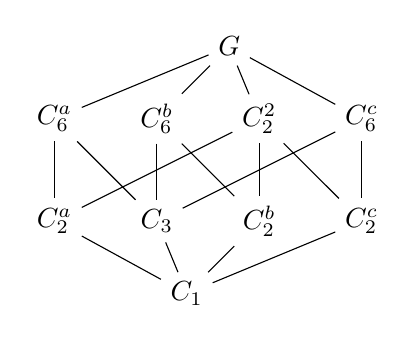
\begin{tikzpicture}[node distance=1.3cm]
        \node(G)[midway]{$G$};
        \node(C6b)[below left of =G]{$C_6^{b}$}; \node(C6a)[left of=C6b]{$C_6^{a}$};  
        \node(C22)[right of=C6b]{$C_2^{2}$};    \node(C6c)[right of=C22]{$C_6^{c}$};
        \node(C2a)[below of=C6a]{$C_2^{a}$};    \node(C3)[below of=C6b]{$C_3$};
        \node(C2b)[below of=C22]{$C_2^{b}$};    \node(C2c)[below of=C6c]{$C_2^{c}$};
        \node(C1)[below left of=C2b]{$C_1$};
        \draw(G)--(C6a);    \draw(G)--(C6b);    \draw(G)--(C6c);    \draw(G)--(C22);
        \draw(C6a)--(C2a);  \draw(C6a)--(C3);
        \draw(C6b)--(C2b);  \draw(C6b)--(C3);
        \draw(C6c)--(C2c);  \draw(C6c)--(C3);
        \draw(C22)--(C2a);  \draw(C22)--(C2b);  \draw(C22)--(C2c);
        \draw(C2a)--(C1);   \draw(C2b)--(C1);   \draw(C2c)--(C1);   \draw(C3)--(C1); 
    \end{tikzpicture}
    \end{figure}
    %There is a Brauer relation coming from the $C_2 \times C_2$-quotient, given by $$\Psi = C_3 - C_6^a - C_6^b - C_6^c + 2G.$$ 
    
    Consider an order $6$ character $\rho_a$ of $G$ with $C_2^{a}$ in its kernel. This has $\bQ(\rho_a) = \bQ(\zeta_6) = \bQ(\sqrt{-3})$. Let $\tau$ generate $\Gal(\bQ(\rho_a) / \bQ)$. One has
    \begin{equation}\label{ex1-rel}\tag{\textdagger}
    \Ind_{C_2^{a}}^G \trivial  \ominus \Ind_{C_6^{a}}^G \trivial \ominus \Ind_{C_2^{2}}^G \trivial \oplus \Ind_G^G \trivial \simeq \rho_a \oplus \rho_a^{\tau} .
    \end{equation}
    Let $E / \bQ$ be a semistable elliptic curve. To apply Theorem \ref{thm_positive_rank}, we need to compute
    \begin{equation}\label{ex1}\tag{*} 
        \frac{C_{E / F^{C_2^a}} C_{E / \bQ} }{C_{E / F^{C_6^a}} C_{E / F^{C_2^2}}} = 
        \frac{C_{E / L} C_{E / \bQ}}{C_{E / L^{C_3}} C_{E / L^{C_2}}}
    \end{equation} 
    where $L = F^{C_2^a}$ has $\Gal(L / \bQ) = C_6$, and check whether it is a norm from $\bQ(\sqrt{-3})$. This is a product of local Tamagawa numbers, as the minimal differential terms are $1$ when $E / \bQ$ is semistable (Lemma \ref{lem_Dterms}(i)). 
    
    One needs to compute these locally for each $p \in \bQ$. If $E / \bQ_p$ has good reduction, then the Tamagawa numbers at all places above $p$ in the subfields of $L$ are $1$. Suppose that $E / \bQ_p$ has split multiplicative reduction at $p$. Let $n = v_p(\Delta_E)$. For $H \leq G$, the Tamagawa number at a prime $\fp$ above $p$ in $L^H$ is given by $c_{\fp}(E / L^H) = e_{\fp / p} n$, where $e_{\fp \mid p}$ is the ramification degree. Thus the computation of Tamagawa numbers depends on the choice of decomposition group $D_p \leq C_6$ (to count the number of primes above $p$ in a given subfield) and the choice of inertia group $I_p \leq C_6$ (to compute the ramification indices). The following table describes the product of Tamagawa numbers at places above $p$ in our expression, for varying $D_p$ and $I_p$. We let $C_{\fp \mid p}(E / L^H) = \prod_{\fp \mid p}c_{\fp}(E / L^H_{\fp})$ for $H \leq \Gal(L / \bQ)$, and write $C_p = c_p(E / \bQ)C_{\fp \mid p}(E / L) \big/ C_{\fp \mid p}(E / L^{C_3})C_{\fp \mid p}(E / L^{C_2})$. 
    \[
    \begin{array}{c c c c c c c}
        D_p & I_p & c_p(E / \bQ) & C_{\fp \mid p}(E / L^{C_3}) & C_{\fp \mid p}(E / L^{C_2}) & C_{\fp \mid p}(E / L) & C_p\\ 
        \hline
        C_1 & C_1 & n & n^2 & n^3 & n^6 & \square\\
        C_2 & C_1 & n & n & n^3 & n^3 & \square\\
        C_3 & C_1 & n & n^2 & n & n^2 & \square \\
        C_6 & C_1 & n & n & n & n & \square \\
        C_2 & C_2 & n & 2n & n^3 & (2n)^3 & \square \\
        C_6 & C_2 & n & 2n & n & 2n & \square \\
        C_3 & C_3 & n & n^2 & 3n & (3n)^2 & 3\cdot\square \\
        C_6 & C_3 & n & n & 3n & 3n & \square\\
        C_6 & C_6 & n & 2n & 3n & 6n & \square
    \end{array}
    \]

    In all cases we see that $C_p$, the contribution of Tamagawa numbers above $p$, is a norm form $\bQ(\sqrt{-3})$. It is not too hard to check that this is also the case when $E / \bQ_p$ has non-split multiplicative reduction. Therefore the expression in \eqref{ex1} is always a norm from $\bQ(\rho_a)$. This is an example of a more general phenomenon; for cyclic groups and semistable elliptic curves we always get a norm. This follows from  Theorem \ref{thm_consistent_cyclic}, which is proven in \S\ref{sec-cyclic}.
    %and $F / \bQ$ an abelian extension with $G = \Gal(F / \bQ)$. We claim that $C(\Theta) \in \fieldnorm{\rho_a}$, for all such $E$. Since each subgroup in $\Theta$ contains $C_2^{a}$, we have that $C(\Theta)$ equals $C(\Theta / C_2^{a})$ where $\Theta / C_2^{a} \in \B(G / C_2^{a}) = \B(C_6)$.  Now $\Theta / C_2^{a}$ is a $\chi_6$-relation, where $\chi_6 = \rho_a^{C_2^a}$ is a faithful order $6$ character of $C_6$, with $\bQ(\chi_6) = \bQ(\rho_a)$. But for cyclic groups we always get norm relations; by Theorem \ref{thm_consistent_cyclic}, $C(\Theta / C_2^{a}) \in \fieldnorm{\rho_a}$.

    But! Observe that{\footnote{this is called a Brauer relation, see Definition \ref{def-brauer}}} 
    \[ \Ind_{C_3}^G \trivial \ominus \Ind_{C_6^a}^G \trivial \ominus \Ind_{C_6^b}^G \trivial \ominus \Ind_{C_6^c}^G \trivial \oplus (\Ind_G^G \trivial)^{\oplus 2} = 0 \]
    as a virtual permutation representation. We can append this to the left hand side of \eqref{ex1-rel}. Then Theorem \ref{thm_positive_rank} asks us to compute 
    \begin{equation}\label{ex1-rel2}\tag{**}
    \left(\frac{C_{E / F^{C_2^a}} C_{E / \bQ} }{C_{E / F^{C_6^a}} C_{E / F^{C_2^2}}}\right) \cdot \left( \frac{C_{E / F^{C_3}} C_{E / \bQ}^2}{C_{E / F^{C_6^a}}C_{E / F^{C_6^b}}  C_{E / F^{C_6^c}} } \right). 
    \end{equation}
    
    We can find instances where the second factor is not a norm from $\bQ(\sqrt{-3})$. Indeed suppose $E / \bQ$ has split multiplicative reduction at a prime $p$ with $D_p = G$, $I_p = C_6^b$ (assuming tamely ramified, one can take a prime $p$ such that $6 \mid p^2 - 1$, e.g. $p = 5$). Let $v_p(\Delta_E) = n$. Then there is only one prime above $p$ in each subfield. Suppose $E$ has good reduction at all other primes (or multiplicative reduction at primes that are totally split in $F / \bQ$ would also be fine).
     Then our expression \eqref{ex1-rel2} is equal to
     \[ \frac{(6n)(n)}{(2n) (3n)} \cdot \frac{(2n)(n)^2}{(2n)(n)(2n)} = \frac{1}{2} \cdot \square,\] 
     but $\frac{1}{2}$ is not a norm in $\bQ(\sqrt{-3})$. Hence one must have $\rk E / F > 0$. 
\end{example}

\begin{example}[Dihedral]
    Let $q_1, q_2$ be odd primes. Consider $G = D_{2 q_1 q_2}$ the dihedral group of order $2 q_1 q_2$. 
    Let $\rho$, $\tau_1$, $\tau_2$ be two-dimensional irreducible representations of $G$ corresponding to rotating a $(q_1 q_2)$-gon by $2 \pi / q_1 q_2$, $2 \pi / q_1$, $2 \pi q_2$ respectively. The Galois conjugates of these representations, as well as the trivial $\trivial$ and sign $\epsilon$, yield all the irreducible representations of $G$. One has
    \begin{table}[H]
        \centering
    \begin{tabular}{l}
        $\Ind_{C_2}^G \trivial \simeq \trivial \oplus \repnorm{\tau_1} \oplus \repnorm{\tau_2} \oplus \repnorm{\rho},$ \\
        $\Ind_{D_{2 q_1}}^G \trivial \simeq \trivial \oplus \repnorm{\tau_2}$,\\
        $\Ind_{D_{2 q_2}}^G \trivial \simeq \trivial \oplus \repnorm{\tau_1}$.
    \end{tabular}
\end{table}
% There is an irreducible representation $\rho$ of $G$, obtained by inducing a linear order $q_1 q_2$ faithful representation from $C_{q_1 q_2}$. Thus $\rho$ is of degree $2$ and $\bQ(\rho) = \bQ(\zeta_{q_1 q_2})^{C_2}$. Then $\rho$ has $\frac{(q_1 - 1)(q_2 - 1)}{2}$ Galois conjugates, and so $\repnorm{\rho}$ is of dimension $2 \cdot \frac{(q_1 - 1)(q_2 - 1)}{2}$. 
Thus there is a $\rho$-relation $$\Theta = C_2 - D_{2 q_1} - D_{2 q_2} + G, \qquad \bC[G / \Theta] \simeq \repnorm{\rho}.$$ 

    Suppose that $E / \bQ$ is semistable. Recall that $C(\Theta) = \prod_p C_{\fp \mid p}(\Theta)$. Suppose that $E / \bQ_p$ has split multiplicative reduction, with $n = v_p(\Delta_E)$. Then by Proposition \ref{prop_local_fns}, $C_{\fp \mid p} = (D_p, I_p, en)$. Corollary \ref{cor-odd-decomp} implies that $C_{\fp \mid p}(\Theta)$ is a norm from the quadratic subfields of $\bQ(\rho)$ whenever $|D_p|$ is odd. In fact, ranging over all possible $D_p$ and $I_p$, a case by case analysis yields that $C_{\fp \mid p}(\Theta)$ is non-square only when the decomposition group is $D_{2 q_1}$ or $D_{2 q_2}$ (and $I_p$ is non-trivial). 

    For example, let $p$ have decomposition group $D_{2 q_1}$ and inertia group $C_{q_1}$. We use Exercise \ref{ex-counting} to compute $(D_p, I_p, en)$ on each subgroup in $\Theta$:
        \begin{itemize}[--]
            \setlength\itemsep{0em}
            \item The action of $D_{2 q_1}$ on $C_2 \backslash G$ yields $1$ orbit of size $C_{q_1}$ (the orbit of the identity) and $\frac{q_2 - 1}{2}$ orbits of size $2q_1$ (coming from $C_2$ acting faithfully on $C_{q_2}$). The size of the inertia sub-orbits is $q_1$. Hence $C_{\fp \mid p}(C_2) = (q_1 n)^{1 + \frac{q_2 - 1}{2}}$.
            \item The action of $D_{2 q_1}$ on $D_{2 q_1} \backslash G$ yields the same number of orbits as above, but now the action of $C_{q_1} \leq D_{2 q_1}$ is trivial and the size of the inertia sub-orbits are all $1$, so that $C_{\fp \mid p}(D_{2 q_1}) = n^{1 + \frac{q_2 - 1}{2}}$.
            \item The action of $D_{2 q_1}$ on $D_{2 q_2} \backslash G$ yields one orbit of size $q_1$, with the inertia sub-orbit also of size $q_1$, hence $C_{\fp \mid p}(D_{2 q_2}) = q_1 n$.
        \end{itemize}
    In total,
    \[ C_{\fp \mid p}(\Theta) = \frac{(q_1 n )^{1 + \frac{q_2 - 1}{2}} (n)}{(n)^{1 + \frac{q_2 - 1}{2}} (q_1 n)} = q_1^{\frac{q_2 - 1}{2}} .\] 
    By symmetry, taking the decomposition group to be $D_{2 q_2}$ and inertia group $C_{q_2}$, one has 
     $C_{\fp \mid p}(\Theta) = q_2^{\frac{q_1 - 1}{2}}$.

    So let $E / \bQ$ have split multiplicative reduction at $p$ with decomposition group $D_{2 q_1}$ and inertia group $I_p = C_{q_1}$, and good reduction at all other primes. Further suppose that $q_1, q_2 \equiv 3 \pmod 4$ and that $\legendre{q_1}{q_2} = -1$. Then $\bQ(\sqrt{q_1 q_2}) \subset \bQ(\rho)$ but $C_{\fp \mid p}(\Theta) \not\in N_{\bQ(\sqrt{q_1 q_2}) / \bQ}(\bQ(\sqrt{q_1 q_2})^{\times})$. Indeed, one has $C_{\fp \mid p}(\Theta) \equiv q_1 \mod (\bQ^{\times})^2$, but $q_1$ is not the norm of an element of $\bQ(\sqrt{q_1 q_2})$, since $z^2 q_1 = x^2 - q_1q_2 y^2$ for $x,y,z \in \bZ$ implies $q_1 = \square \pmod {q_2}$, a contradiction. Thus $\rk E / F > 0$.

    This rank growth is predicted by root number computations also, however. Assume that $F / \bQ$ is totally real. Then $w(E / F^H) = (-1)^{[F^H \colon \bQ] + | H \backslash G / D_p|}$ by Proposition \ref{compute-root}. Thus
    \begin{itemize}[--]
        \setlength\itemsep{0em}
        \item $w(E / \bQ) = (-1)^2 = 1$,
        \item $w(E / F^{C_2}) = (-1)^{q_1 q_2} (-1)^{1 + \frac{q_2 - 1}{2}} = (-1)^{\frac{q_2 - 1}{2}}$,
        \item $w(E / F^{D_{2 q_1}}) = (-1)^{q_2}(-1)^{1 + \frac{q_2 - 1}{2}} = (-1)^{\frac{q_2 - 1}{2}},$
        \item $w(E / F^{D_{2 q_2}}) = (-1)^{q_1}(-1) = 1$. 
    \end{itemize}
    Therefore we must have $\rk E / F^{C_2}$, $\rk E / F^{D_{2q_1}} > 0$, so $\rk E / F > 0$. 
    Using the properties in Proposition \ref{compute-root-twist}, the computations of the root numbers for the subfields implies that 
    \[ w\left(E / \bQ, \repnorm{\tau_1}\right) = 1, \quad w\left(E / \bQ, \repnorm{\tau_2}\right) = -1, \quad w\left(E / \bQ, \repnorm{\rho}\right) = 1, \]
  and in particular there is an irreducible self-dual Artin rep $\tau'$ with $w(E / \bQ, \tau') = -1$ (some irreducible consistent of $\repnorm{\tau_2}$). In particular the parity conjecture for twists implies that $\left\langle \repnorm{\tau'}, E(F)_{\bC} \right\rangle > 0$. 
    
  
  {\color{red} maybe I could add how this suggests we throw in a $q_1$ for the regulators and then everything is fine }
\end{example}

\begin{example}[Additive reduction example]



\end{example}


\newpage
\section{Forcing points of infinite order}
In [Dok-Wier-Ev], they establish a (dependent on some conjectures) test for forcing a point of infinite order.

\begin{thm}\label{dew-thm}
    Let $E / \bQ$ be an elliptic curve, $F / \bQ$ a Galois extension with Galois group $G$, $\rho$ an irreducible representation of $G$ and 
    \begin{equation}\label{rho-reln}
        \left(\bigoplus_{g \in \Gal(\bQ(\rho) / \bQ)} \rho^g\right)^{\oplus m(\rho)} = 
        \left(\bigoplus_i \Ind_{H_i}^G \trivial \right) \ominus \left(\bigoplus_j \Ind_{H_j'}^G \trivial \right),
    \end{equation}
    for some $m(\rho) \in \bZ$ and subgroups $H_i, H_j' \leq G$. 

    If either $\prod_i C(E / F^{H_i}) / \prod_j  C(E / F^{H_j'})$ is not a norm from some quadratic field $\bQ(\sqrt{D}) \subset \bQ(\rho)$, or if it is not a rational square when $m(\rho)$ is even, then $E$ has a point of infinite order over $F$.
\end{thm}

In this paper, they give two examples of applications of this theorem. Of course, another means of forcing infinite order is via root numbers. We are currently unsure as to whether this norm test is weaker/equivalent/stronger than the test of root numbers. For example, in odd order extensions, root numbers don't tell us anything. We show in the next section that this norm test doesn't either, that is, the product of Tamagawa numbers is always a norm.

\vspace{1em}

As discussed in section \ref{D-loc}, the function on $B(G)$ sending $H \mapsto C(E / F^H)$ is the product of local functions depending on the decomposition group $D_p$ at a prime $p$. We denote each of these as $(D_p, I_p, \psi_p)$, as in definition \ref{D-I-fn}. Then the product of Tamagawa numbers in \ref{dew-thm} is the evaluation of $\prod_p (D_p, I_p, \psi_p)$ on $\sum_i H_i - \sum_j H_j'$.

If we are interested in evaluating each $(D_p, I_p, \psi_p)$ individually, then we have some freedom to change our field extension to make computations easier. In particular, 

\begin{lemma}\label{DeqI}
    In an odd degree unramified extension, Tamagawa numbers change only up to squares. In particular, if $[D_p \colon I_p]$ is odd, then $(D_p, I_p, \psi_p) \sim_{\rho} (D_p, D_p, \psi_p)$ for any $\rho$ with $\bQ(\rho)$ even. 
\end{lemma}

\begin{proof}
    Yadada
\end{proof}


%Let $F_i = F^{H_i}$, $F_j = F^{H_j'}$.
%Note that $$\prod_i C(E / F_i) / \prod_j  C(E / F_j')  = \prod_p \left(\prod_i  C_{p}(E / F_i) /  \prod_j C_{p}(E / F_j')\right)$$
%where $C_p(E / F_i) =\prod_{v | p} c_v(E / F_i)\cdot |\omega / \omega_{v, \min}|$.

%Let $D_p$, $I_p$ be the decomposition and inertia subgroups of $G$ at $p$.
%The function on the Burnside ring of $G$ sending $H$ to $C_p(E / F^H)$ is then of the form $(D_p, I_p, \psi_p).$ 


\subsection{Compatibility in odd order extensions}

 Let $E / \bQ$ be an elliptic curve. Let $F / \bQ$ be an extension of \textbf{odd order} with Galois group $G$. Consider a representation $\rho \in R(G)$ and the expression as in theorem \ref{thm_positive_rank}. The $m$ occurring in this expression divides $|G|$, hence is odd. The theorem then states that if the corresponding product of fudge factors $C_{E / \cdot}$ is not a norm from a quadratic subfield $\bQ(\sqrt{D}) \subset \bQ(\rho)$, then $E / F$ must have infinite order. 

 In this section, we show under some restrictions for $E$ that we can never use this test to force positive rank.

\begin{thm}
    Suppose that the primes of additive reduction of $E$ are at worst tamely ramified in $F / \bQ$ (and $\geq 5$). 
    Then for any representation $\rho$ of $G$ and any expression as in theorem \ref{thm_positive_rank}, the corresponding ratio of fudge factors is a norm from any quadratic subfield of $\bQ(\rho)$.
    Equivalently, the function $H \mapsto C(E / F^H)$ is trivial on $\rho$-relations. 
\end{thm}

If $\bQ(\rho) = \bQ$ there is nothing to prove. 
Thus we assume $[\bQ(\rho) \colon \bQ] > 1$. Then this index is even. Indeed, since $G$ has odd order, all its characters are complex, so there is an element $\sigma \in \Aut(\bQ(\rho) / \bQ)$ that acts by complex conjugation (i.e. is of order $2$). Therefore there is a quadratic subfield $\bQ(\sqrt{D}) \subset \bQ(\rho)$. Choose any such quadratic subfield. Replacing $\rho$ by the sum of its conjugates by elements of $ \Gal(\bQ(\rho) / \bQ(\sqrt{d}))$, we may assume that $\bQ(\rho) = \bQ(\sqrt{D})$. Let $\tau$ be the generator of $\Gal(\bQ(\sqrt{D}) / \bQ)$. 

Let $k$ be the smallest integer such that $\bQ(\sqrt{D}) \subset \bQ(\zeta_k)$. Then $k$ divides the exponent of $G$, hence is odd.

\vspace{1em}
Let us break up the function $C \colon H \mapsto C(E / F^H)$ into $C = \prod_p  C_p \cdot d_p$ where
        \[ C_p(H) =  C_p(E / F^H) := \prod_{v | p}  c_v(E / F^H) , \qquad d_p(H) = \prod_{v | p} \left|\frac{\omega}{\omega_{v}^{\min}}\right|_v . \]
We will observe later that for each reduction type, $C_p$ and $d_p$ are $D_p$-local functions. 
 
We prove that each $C_p \sim_{\rho} 1$ and $d_p \sim_{\rho} 1$ for all primes $p$. We do this by considering serpately each reduction type. Since we deal with each local factor individually, we may assume that $D_p = I_p$ by theorem \ref{DeqI}. {\color{red} does that include the dv terms???}

\subsubsection*{Good reduction}
If $E / \bQ$ has good reduction at $p$, then it has good reduction at all primes lying above $p$ in subfields of $F$. Then the tamagawa number is always one, as well as $\left|\omega / \omega_{v}^{\min}\right|_v$ for any place $v \mid p$ in an intermediate field. Therefore $C_p$, $d_p \sim_{\rho} 1$.

\subsubsection*{Multiplicative reduction}

If $E / \bQ_p$ has multiplicative reduction, then as in the good reduction case one has $\left|\omega / \omega_{v}^{\min}\right|_v = 1$ for any place $v \mid p$ in an intermediate field. Thus $d_p \sim_{\rho} 1$.
For the Tamagawa numbers, we consider non-split/ split reduction separately.
\vspace{1em}

\noindent\underline{\textit{Non-split multiplicative reduction}}

Let $E / \bQ_p$ have non-split multiplicative reduction. Since $D_p = I_p$, all primes above $p$ have residue degree $1$. Then the reduction at places above $p$ remains non-split in all intermediate subfields.
It follows that 
\[ C_p = (D_p, \alpha) \]
where $\alpha$ is the constant function on $B(D_p)$ with $\alpha \in \{1, 2\}$, depending on $\ord_p(\Delta)$ being even or odd. 
We prove a more general lemma that $D_p$-local constant functions are trivial on $\rho$-relations.

\begin{lemma}\label{const-fns}
Let $G$, $\rho$ be as above. The function $(D_p, \alpha)$ for $\alpha \in \bQ^{\times}$ satisfies $(D_p, \alpha) \sim_{\rho} 1$.  
\end{lemma}   

\begin{proof}
    The function $(D_p, \alpha)$ on $B(G)$ sends $H \leq G$ to $\alpha^{| H \backslash G / D_p|}$. Thus if $\Theta = \sum_i n_i H_i$ is a $\rho$-relation, $(D_p, \alpha)(\Theta) = \alpha^{ \sum_i n_i \cdot | H_i \backslash G / D_p|}$. We show that $\sum_i n_i \cdot | H_i \backslash G / D_p|$ is even. 

    %Since $G$ is odd, each $| H_i \backslash G / D_p|$ is odd. On the other hand, $\rho \oplus \tau(\rho)$ has even dimension. Therefore $\sum_i |n_i|$ is even. 
    One has $\Res_D \Theta = \sum_i n_i \sum_{x \in H_i \backslash G / D} D \cap H^{x^{-1}}$ and the permutation representation $\bC[\Res_D \Theta]$ of $D$ is isomorphic to $\Res_D (\rho \oplus \tau(\rho))$. In particular the dimension of this permutation representation is even. The dimension is $\sum_i n_i \sum_{x \in H_i \backslash G / D} [D \colon D \cap H^{x^{-1}} ]$. Since each $[D \colon D \cap H^{x^{-1}} ]$ is odd, this implies there are an even number of terms in the summation, i.e. that $\sum_i n_i \cdot | H_i \backslash G / D_p|$ is even. 
    
\end{proof}

\noindent\underline{\textit{Split multiplicative reduction}}

Now suppose $E / \bQ_p$ has split multiplicative reduction. The reduction type remains split at all places above $p$ within sub-extensions of $F / \bQ$. Let $\ord_p(\Delta) = n$. Then 
\[ C_v = (D_p, I_p, en). \]
Since the $n$ factor is constant by lemma \ref{const-fns} we have $(D_p, I_p, en) \sim_{\rho} (D_p, I_p, e)$.
This is a $D_p$-local function.
The following result shows that if $\bQ(\Res_{D_p}\rho ) = \bQ$, then $(D_p, I_p, e) \sim_{\rho} 1$.

\begin{lemma}\label{rational-res}
    Let $G, \rho$ be as above, $D_p \leq G$. Let the exponent of $D_p$ be $b$. If $k \nmid b$, then $(D_p, I_p, e) \sim_{\rho} 1$. 
\end{lemma}

\begin{proof}
    Note that $\bQ(\Res_{D_p}{\rho}) \subset \bQ(\zeta_b) \cap \bQ(\rho) \subset \bQ(\zeta_b)$. Then $\bQ(\rho) \subset \bQ(\zeta_b) \implies k \mid b$ by minimality of $k$. Thus, if $k \nmid b$, one has $\bQ(\rho) \not\subset \bQ(\zeta_b)$, so $\bQ(\Res_{D_p} \rho) = \bQ$ and $\Res_{D_p} \rho = \tau (\Res_{D_p} \rho)$. 
    
    Let $\Theta$ be a $\rho$-relation. It follows that every rational representation that is a summand of $\bC[\Res_{D_p} \Theta]$ arises with multiplicity two. 
    Thus, there is a $(\Res_{D_p}\rho$)-relation $\Theta ' $ such that $\bC[\Res_{D_p} \Theta] \simeq \bC[2 \Theta']$. Then $\Psi = \Theta - 2 \Theta'$ is a Brauer relation for $D_p$. We have 
    \[(D_p, I_p, e)(\Theta) = (D_p, I_p, e)(\Psi) \cdot (D_p, I_p, e)(2 \Theta') = (D_p, I_p, e)(\Psi)  \cdot ((D_p, I_p, e)(\Theta'))^2 = 1\]
    as a function to $\bQ^{\times} / \bQ^{\times}$. Indeed $(D_p, I_p, e)(\Psi) = 1$ on Brauer relations, as per example \ref{trivial-on-brauer} (noting that $D_p$ is odd). Thus $(D_p, I_p, e) \sim_{\rho} 1$.
\end{proof}

We have $D_p = I_p = P_p \ltimes C_l$, where $P_p \triangleleft I_p$ is wild inertia, and $C_l = I_p / P_p$ is the tame quotient. $C_l$ is a cyclic group, with $l \mid p^f - 1 = p - 1$. By the previous result, it is only of interest to consider decomposition groups $D_p = P_p \ltimes C_l$, with $k \mid p^u l$ for some $u \geq 0$. 

Now, $(D_p, I_p, e)(\Theta)$ is the product of ramification indices at primes above $p$. We separate the $p$-part and tame part of this expression.
Recall that the ramification index of a place $w$ above $p$ corresponding to the double coset $H_i x D_p$ has ramification degree $e_w = \frac{|I_p|}{|H_i \cap I_p^x|} =\frac{|I_p|}{|I_p \cap H^{x^{-1}}|}$.
This is the dimension of the permutation representation $\bC[D_p / D_p \cap H^{x^{-1}}]$.
Let  $D_p \cap H^{x^{-1}} = P' \ltimes C_a$ where $P' \leq P$ and $a | l$. Then the ramification index is $\frac{|P|}{|P'|}\cdot \frac{l}{a}$. 


Consider taking fixed points $$\bC[D_p / D_p \cap H^{x^{-1}}]^{P_p} \simeq \bC[D_p / P_p (D_p \cap H^{x^{-1}})] \simeq \bC[D_p / P_p \ltimes C_a].$$ This permutation representation has dimension $\frac{l}{a}$, so we've killed off the $p$-part. 
Then $$\bC[\Res_{D_p} \Theta]^{P_p} \simeq \left(\Res_{D_p} \rho \oplus \tau(\rho)\right)^{P_p}$$
and we can consider these as representations of $D_p / I_p = C_l$. 
Consider the function $g$ on $B(C_l)$ sending $H$ to $[C_l \colon H]$. 
It follows that $(D_p, D_p, e)(\Theta)$ differs from $g(P_p \cdot \Res_{D_p}\Theta / P_p)$ up to a factor of $p$. 

%$(C_l, C_l, e)$ evaluated at $P_p \cdot \Res_{D_p}\Theta / P_p$ equals $(D_p, D_p, \psi_p)$ evaluated at $\Res_{D_p} \Theta$ modulo squares up to (possibly) a factor of $p$.

Crucially, this factor of $p$ doesn't matter:

\begin{lemma}
    Let $K = \bQ(\sqrt{D})$ be a quadratic field, contained in the minimal cyclotomic field $\bQ(\zeta_k)$ with $k$ odd. Let $k \mid p^u l $, for some $u \geq 0$ and $l$ such that $p \equiv 1 \pmod l$. Then $p$ is the norm of an element from $K^{\times}$.
\end{lemma}

\begin{proof}
    Since $k$ is odd, it is clear that $D = \prod_{q | k} q^*$, the product being taken over primes dividing $k$. Note that if $q \not= p$, then since $q \mid l$, we have $p \equiv 1 \pmod l \implies p \equiv 1 \pmod q$. By theorem \ref{p-one-mod-disc},  $p$ is the norm of a principal fractional ideal of $K$. If $K$ is imaginary, then $p$ is the norm of an element of $K$. Else, we invoke theorem \ref{p-norm-elem-1} or theorem \ref{p-norm-elem-2}.
    %We show that $p$ has inertial degree $1$ in the extended genus field $E^{+} = K(\{\sqrt{q^*} \colon q | k \})$ of $K$ ({\color{red} cf. appendix}).
    %If $q \not= p$ then $q \mid l$, so $p \equiv 1 \pmod l$. Therefore $p$ splits in any quadratic subfield of $E^{+}$ of discriminant not divisible by $p$. Else, $p$ ramifies in any quadratic subfield with discriminant divisible by $p$. Thus it is clear that $p$ has inertial degree $1$ in $E^{+}$, hence also in the genus field $E$, and it follows from theorem \ref{p-principal} that $p$ is the norm of a principal ideal.  Else, we invoke theorem \ref{minus-one-norm}.
\end{proof}

Thus, we only need to worry about the tame part of our ramification indices, and the triviality of the function $g$ on $B(C_l)$. If $k \nmid l$, then $\phi = (\Res_{D_p} \rho)^{P_p}$ (viewed as a representation on $D_p / P_p$) has rational character. Therefore, arguing as in lemma \ref{rational-res}, $g \sim_{\phi} 1$ as a function to $\bQ^{\times} / \bQ^{\times 2}$.
Therefore we may assume that $k \mid l$ and that $\phi$ has $\bQ(\phi) = \bQ(\rho) = K$.

\begin{prop}
    Let $k \mid l$, then one has $g \sim_{\phi} 1$.   
\end{prop}

\begin{proof}
    Let $\Psi$ be a $\phi$-relation. One may write $\phi \oplus \tau(\phi) = \bC[\Psi] = \sum_{l' \mid l}{a_{l'}} \chi_{l'}$ where $a_{l'} \in \bZ$ and $\chi_{l'}$ are defined in example \ref{cyclic-relns}. Writing each $\chi_{l'}$ in terms of permutation representations as in the example, one obtains an expression for $\bC[\Psi]$, noting this is exact since cyclic groups have no Brauer relations.

    Evaluating $g$ on $\chi_{l'}$ is trivial unless $l' = q^a$ for some $q$ prime, $a \geq 1$. Indeed, if $l' = p_1^{e_1} \cdots p_r^{e_r}$ , with $r \geq 2$ and $e_i \geq 1$, then {\color{red} maybe expand on this}
    \[ \prod_{l'' \mid l'} (l'')^{\mu(l' / l'')} = \prod_{j_1, \ldots j_r \in \{0,1\}^r } \left(p_1^{e_1 - j_1} \cdots p_r^{e_r - j_r}\right)^{\# j_i = 1} = \prod_{i = 1}^r \left(\frac{p_i^{e_i}}{p_i^{e_i - 1}}\right)^{\sum_{ j = 0}^{r - 1} \binom{r-1}{j} (-1)^j} = 1. \]
    On the other hand,
    \[ \prod_{l' \mid q^a} (l')^{\mu(q^a / l')} = q .\]
    
    We claim that $k \nmid l'$ implies $a_{l'}$ is even. The irreducible representations of $C_l$ over $\bQ(\phi)$ are given by the orbits of the complex irreducible characters of $C_l$ acted upon by $H = \Gal (\bQ(\zeta_l) / \bQ(\phi))$. One has $\chi_{l'} = \widetilde{\varphi_{l'}}$ where $\bQ(\varphi_{l'}) = \bQ(\zeta_{l'})$. If $ k \nmid l'$ then $\bQ(\phi) \not\subset \bQ(\zeta_{l'})$, so that $B = \Gal(\bQ(\zeta_l) / \bQ(\zeta_{l'})) \not\leq H$. Then $\bQ(\phi) \cap \bQ(\zeta_{l'}) = \bQ$ so $BH = \Gal(\bQ(\zeta_l) / \bQ)$. Then the orbit of $\varphi_{l'}$ under $H$ is fixed by $BH$, hence is rational. It follows that $\langle \phi, \varphi_{l'} \rangle = \langle \tau(\phi) , \varphi_{l'} \rangle$ so that $a_{l'}$ is even.  

    Thus we can only possibly get something interesting if $k = q$ is a prime. But then $q$ is a norm from $\bQ(\sqrt{q^*})$ by corollary \ref{p-principal}. 
\end{proof}

\subsubsection{Additive reduction}

Now suppose that $E / bQ_p$ has additive reduction. In this case, assume that $p \geq 5$ is at worst tamely ramified in $F / \bQ$. This ensures that $D_p = I_p = C_l$ is cyclic, and $l \mid p - 1$.

This time the terms involving the minimal differentials are not trivial. 
Let $n = \ord_p(\Delta_E)$. 
Consider a place $w$ of $F^H$ over $p$ with ramification degree and inertial degree $e_w$, $f_w$ over $\bQ$. Then $\Delta_E$ has valuation $n e_w$ in $F^H$. It follows that $\Delta_{E,w}^{\min}$ has valuation $n e_w - 12 \cdot \floor{e_w n /12}$. Therefore

%\[ \left|\frac{\Delta_{E}}{\Delta_{E, w}^\min} \right|_w = p^{f_w 12 \cdot \floor{e_w n / 12}} \implies 
%       \left|\frac{\omega}{\omega_{w}^\min} \right|_w = p \]

{\color{red} first say something about how dv terms go away }


\noindent\underline{\textit{Potentially multiplicative reduction}}

Suppose that $E / \bQ_p$ has Kodaira type $I_n^*$. For a tamely ramified finite extension $K' / \bQ_p$ with ramification degree $e$, $E / K'$ has Kodaira type $I_{en}^*$ if $e$ is odd, and type $I_{en}$ if $n$ is even. Thus in odd degree extensions the reduction type will stay potentially multiplicative.
One has that $v_{K'}(\Delta_{E / K'}) = e v_p(\Delta) - 12\floor{e / 2}$.



{\color{red} TO DO}
\vspace{10em}


\noindent\underline{\textit{Potentially good reduction}}

\begin{lemma}
    Consider $M / L$ a field extension. Let $E / L$ be an elliptic curve, $v$ a finite place of $L$ and $w$ a finite place of $M$ with $w \mid v$. Let $\omega_v$ and $\omega_w$ be the minimal differentials for $E / L_v$ and $E / M_w$ respectively. 
    
    Then, if $E / K_v$ has potentially good reduction and the residue characteristic is not $3$ or $2$, one has
    
    \[ \left|\frac{\omega_v}{\omega_w} \right|_{w} = q^{\floor{\frac{e_{F / K} \cdot \ord_v(\Delta_{E, v}^{\min})}{12}}}, \]
    where $q$ is the size of the residue field at $w$.
\end{lemma}

We consider $F / \bQ$ with additive potentially good reduction at $p$ . Since $D_p = I_p$, the size of the residue field is $p$ at all intermediate extensions. Let $n = v_p(\Delta)$. Then $n \in \{2,3,4,6,8,9,10\}$.  Consider $(D_p, I_p, \psi_p)$ where $\psi_p(e,f) = p^{\floor{e n / 12}}$. Then $(D_p, I_p, \psi_p) \sim_{\rho} 1$. Indeed, this takes values $1$ or $p$ in $\bQ^{\times} / \bQ^{\times 2}$. But $p \equiv 1 \pmod l$ implies that $p$ is the norm of a principal ideal in $\bQ(\rho)$, and hence the norm of an element, by corollary \ref{p-one-mod-disc} and theorem \ref{minus-one-norm}.

The Tamagawa numbers take a little more work. We use the following description of Tamagawa numbers. %Tim and Vlad reg consts Lemma 3.19

\begin{lemma}
    Let $K' /K / \bQ_p$ be finite extensions and $p \geq 5$. Let $E / K$ be an elliptic curve with additive reduction; 
    \[ E \colon y^2 = x^3 + Ax + B, \]
    with discriminant $\Delta = -16(4 A^3 + 27 B^2)$. Let $\delta = v_K(\Delta)$, and $e = e_{K' / K}$.

    If $E$ has potentially good reduction, then 
        \[
        \begin{array}{l l l l}
            \gcd(\delta e, 12) = 2 & \implies & c_v(E / K') = 1, & \quad (II, II^*) \\
            \gcd(\delta e, 12) = 3 & \implies & c_v(E / K') = 2, & \quad (III, III^*) \\
            \gcd(\delta e, 12) = 4 & \implies & c_v(E / K') = \begin{cases} 1, & \sqrt{B} \notin K'
                                \\ 3, & \sqrt{B} \in K' \end{cases}, & \quad (IV, IV^*) \\
            \gcd(\delta e, 12) = 6 & \implies & c_v(E / K') = \begin{cases} 2, & \sqrt{\Delta} \notin K'
                \\ 1 \ \text{or} \ 4, & \sqrt{\Delta} \in K' \end{cases}, & \quad (I_0^*) \\
            \gcd(\delta e, 12) = 12 & \implies & c_v(E / K') = 1. & \quad (I_0)
        \end{array}
        \]
    Moreover, the extensions $K'(\sqrt{B}) / K'$ and $K'(\sqrt{\Delta}) / K'$ are unramified.
\end{lemma}

So suppose an elliptic curve $E / \bQ$ has additive reduction at $p$, with $p \geq 5$. Then we can write $E \colon y^2 = x^3 + Ax + B$. Let $D = \Gal(F_{\fp} / \bQ_p)$ be the local Galois group at $p$. Assume that $p$ is totally tamely ramified, so that $D = I = C_n$. Since there is no wild ramification, and $f = 1$, this means that $n \mid p - 1$. We consider the contribution corresponding to an irreducible rational character $\chi_d$ of $D$, given by 
\begin{equation}\label{tam-contrib}
\prod_{d ' \mid d} C(E / F_{\fp}^{D_{d'}})^{\mu(d / d')}.
\end{equation}

Observe that in a totally ramified extension of degree coprime to $12$, the Tamagawa number remains the same. If $(12, d) = 1$, then $(12, d') = 1$ for $d' \mid  d$, so the Tamagawa number is constant across subfields $F_{\fp}^{D_{d'}}$. Therefore,
\[\prod_{d ' \mid d} C(E / F_{\fp}^{D_{d'}})^{\mu(d / d')} = C(E / \bQ_p)^{\sum_{d' \mid d} \mu(d / d')} = 1,\]
assuming $d > 1$. 

So we only need to worry about when $3 \mid d$. If we have type $III$ or $III^*$ or $I_0^*$ then the Tamagawa number is still unchanged in any totally ramified cyclic extension of degree dividing $d$. We will treat the other cases separately: 

\vspace{1em}

\noindent\underline{\textit{Type $II$ and $II^*$ reduction:}}

Firstly, suppose that $\delta = 2$, that is we have Type $II$ reduction. If $3 \mid d'$ then $E / F_{\fp}^{D_{d'}}$ has type $I_0^*$ reduction. The Tamagawa number then depends on whether $\sqrt{\Delta} \in \bQ_p$. Since we have additive reduction, we know that $p \mid A$, $p \mid B$. Moreover, $\delta = 2$ implies that $v_p(B) = 1$. Then, $\Delta = p^2\cdot \alpha$, and $\alpha \equiv -27\cdot\square \pmod p$. Therefore $\sqrt{\Delta} \in \bQ_p \iff -3$ is a square $\pmod p$. But this is the case; we assumed $p \equiv 1 \pmod n$, so $p \equiv 1 \pmod 3$. Therefore the Tamagawa number will be $1$ or $4$, which is a square.
If $3 \nmid d'$ then the reduction type over $ F_{\fp}^{D_{d'}}$ is $II$ or $II^*$. Then the Tamagawa number is $1$. Thus in total, we get a square contribution from (\ref{tam-contrib}).

If $\delta = 10$, then $E / F_{\fp}^{D_{d'}}$ has reduction type $I_0^*$ whenever $3 \mid d'$. Once more, $v_p(A), v_p(B) \geq 1$, and $v_p(\Delta) = 10 = \min(3 v_p(A), 2 v_p(B))$ {\color{red} maybe this is suss} $\implies v_p(B) = 5$. Therefore we get $\Delta = p^{10} \alpha$ with $\alpha \equiv -27\cdot\square \pmod p$, and we conclude as above.

\vspace{1em}

\noindent\underline{\textit{Type $IV$ and $IV^*$ reduction:}}

Now, if $E /\bQ_p$ has additive reduction of type $IV$ or $IV^*$, it attains good reduction over any totally ramified cyclic extension of degree divisible by $3$. This could result with $3$ coming up an odd number of times in our Tamagawa number product, when $\sqrt{B} \not\in \bQ_p$. 

%We show that for both types, one has $\sqrt{B} \in \bQ_p$. 
%Indeed, if $\delta = 4$, then $v_p(B) = 2$, and $v_p(A) \geq 2$. 
\vspace{1em}
In summary, 
\begin{equation}
    \prod_{d ' \mid d} C(E / F_{\fp}^{D_{d'}})^{\mu(d / d')}
    = 
    \begin{cases}
        1 & 3 \nmid d, \\
        1 & 3 \mid d, \delta \in \{0, 3, 6, 9\}, \\
        1 \cdot \square & 3 \mid d, \delta \in \{2, 10\}, \\
        3^a \cdot\square, a \in \{0,1\} & 3 \mid d, \delta \in \{4,8\}.
    \end{cases}
\end{equation}

\begin{rem}
   There's no reason why we can't get 3; see elliptic curve 441b1 with additive reduction at $7$ of type IV and Tamagawa number equal to $3$
\end{rem}

However, it turns out we will only get $3$ occurring oddly when $d = 3$. Indeed, one has that $\langle \Ind_{D_{d'}}^D \trivial, \psi_3 \rangle = 1$ if $3 \mid d'$, and $0$ if $3 \nmid d'$, where $\psi_3$ is an irreducible character of $D$ of order $3$. Therefore one sees that the number of places with ramification degree divisible by $3$ cancels unless $d = 3$. Indeed, $\langle \chi_d , \psi_3 \rangle = 0$ unless $d = 3$, 
in which case it is $1$. Therefore (\ref{tam-contrib}) can only be non-square when $d = 3$. {\color{red} then conclude why this is fine}


\section{Brauer Relations}

\newpage
\section{Consistency cases with BSD}
As we discussed in the previous section, our motivation is to use Theorem \ref*{thm_positive_rank} to predict points of infinite order for families of elliptic curves. However, in this section we prove that in several cases the theorem will never make such a prediction. In other words, in such cases, the product 
$$\frac{\prod_i C_{E/F_i}}{\prod_j C_{E/F_j'}}$$ 
is always a norm for every subfield $\QQ(\sqrt{D})\subseteq\QQ(\rho)$.

\subsection{Cyclic Extensions}
In this subsection we prove the following. 
\begin{thm}\label{thm_consistent_cyclic}
    Let $E/\QQ$ be a semistable elliptic curve and let $F$ be a finite cyclic Galois extension $\QQ$ so that $\Gal(F/\QQ)=C_d$ for some $d\geq 2$. Let $\chi$ be a faithful character of $C_d$ (so that $\QQ(\chi)=\QQ(\zeta_d)$), and let $F_i,F'_j\subseteq F$ be such that
    $$\bigoplus_{\mathfrak{g}\in\Gal(\QQ(\zeta_d)/\QQ)}\chi^{\mathfrak{g}}=\bigoplus_i\Ind_{F_i/\QQ}\mathds{1}\ominus\bigoplus_j\Ind_{F'_j/\QQ}\mathds{1}.$$
    Then for any $\QQ(\sqrt{D})\subseteq\QQ(\zeta_d)$,
    $$\frac{\prod_i C_{E/F_i}}{\prod_j C_{E/F_j'}}$$
    is a norm of $\QQ(\sqrt{D})$. Moreover, the contribution is always the square of rational number unless $d=2^n, p^n,2p^n$ for some odd prime $p$.
\end{thm}

The first step in proving Theorem \ref*{thm_consistent_cyclic} is to show that the fields $F_i, F'_j$ exist, and to give a precise description. Recall that for each $k\mid d$ the cyclic group $C_d$ has one unique subgroup of order $k$, which is of course also cyclic. Therefore, for each $k\mid d$, there is one unique subfield $L_k$ of $F$ of degree $k$ over $\QQ$ which is also cyclic. Under the Galois correspondence, this field corresponds to the subgroup $H_k=\Gal(F/L_k)=C_{d/k}$.

To give the required description, we recall that the Möbius function $\mu$ is the function supported on the square-free integers, and $\mu(n)=(-1)^s$ whenever $n$ is square free and $s$ is the number of prime factors of $n$.

\begin{lemma}\label{lem_cyclic_decomp}
    Let $E/\QQ$, $F$ and $\chi$ be as in Theorem \ref*{thm_consistent_cyclic}. Writing characters of $C_d$ additively, we have that
    \begin{equation}\label{eqn_cyclic_relation}
        \sum_{\mathfrak{g}\in\Gal(\QQ(\zeta_d)/\QQ)}\chi^{\mathfrak{g}}=\sum_{k\mid d}\mu(d/k)\Ind_{L_k/\QQ}\mathds{1}.
    \end{equation}
    Furthermore, such an expression is unique.
\end{lemma}

\begin{rem}\label{rem_radical}
    This lemma has an important consequence. Given an integer $d\geq2$, let $\rad(d)=\prod_{p\mid d}p$ be the radical of $d$, and let $K=L_{d/\rad(d)}$ be the unique subfield of $F$ such that $[F:K]=\rad(d)$. For $k\mid d$, $\mu(d/k)\neq 0$ precisely when $[K:\QQ]=\frac{d}{\rad(d)}\mid k$ and therefore the fields appearing in the right hand side of \eqref{eqn_cyclic_relation} are the fields $L_k$ satisfying $K\subseteq L_k\subseteq F$. 
\end{rem}

Following this observation, we will compute the product of the local factors locally for each finite place $\pp$ of $K$ and the places above it in the other fields $L_k\supseteq K$. To that objective, the following notation will be useful.

\begin{notation}\label{not_local_contr}
    Let $E/\QQ$, $F$ and $\chi$ be as in Theorem \ref*{thm_consistent_cyclic}, and let $L_k$ and $K$ be as in Remark \ref*{rem_radical}. For a finite place $\pp$ of $K$, we write
    $$\contr_\chi(\pp)=\prod_{\frac{d}{\rad(d)}\mid k\mid d}C_{\mathfrak{P}\mid\pp}(L_k/K)^{\mu(d/k)}=\prod_{k\mid d}C_{\mathfrak{P}\mid\pp}(L_k/K)^{\mu(d/k)}$$ 
    where the terms in the product are defined as in Notation \ref*{not_contr}. 
\end{notation}

An immediate consequence of the above definition is the fact that 
\begin{equation}\label{eqn_local_contr}
    \prod_{k\mid d}(C_{E/L_k})^{\mu(d/k)}=\prod_\pp\contr_\chi(\pp),
\end{equation}

and therefore we can calculate the product of local terms \textbf{locally}, one prime $\pp$ at a time.

We divide the proof of Theorem \ref*{thm_consistent_cyclic} into two cases: odd and even cyclic extensions. The main idea in both cases is to simplify the general case into smaller cases where we can directly compute $\contr_\chi(\pp)$ for each finite place $\pp$ of $K$. We note that if $E$ has good reduction over $\pp$, then $\contr_\chi(\pp)=1$ and therefore we focus our attention to bad semistable reduction. 

\subsection*{Odd Cyclic Extensions} \label{case_Cp}

For the first case, we assume that $d$ is odd. Following the observation in Remark \ref*{rem_radical}, we need to calculate $\contr_\chi(\pp)$ for each finite place $\pp$ of $K$. To that objective, we first calculate them for ``small'' cases and then we use them for the general case. The following lemmas build on this idea.

\begin{lemma}\label{lem_Cp}
    Let $p$ be a rational prime, $F/K$ a Galois extension of number fields such that $\Gal(F/K)=C_p$ and $E/\QQ$ an elliptic curve. Then 
    $$\frac{C_{E/F}}{C_{E/K}}$$
    is a rational square up factors of $p$.
\end{lemma}

\begin{proof}
    Fix some prime $\pp$ in $K$. Since the extension $L/K$ is cyclic, the splitting behaviour in $L$ is determined by the ramification index $e_\pp$ and the residual degree $f_\pp$. Since $\contr_\chi(\pp)=1$ if $E$ has good reduction at $\pp$ and $E$ is assumed to be semistable, we assume that $E$ has split or non-split multiplicative reduction. The following table records the contribution of $\pp$ dependinng on $e_\pp$ and $f_\pp$, and the entries for split and non-split multiplicative reduction of type $\mathrm{I}_n$ are separated by a ``;''.
    \begin{table}[h!]
        \centering
        \begin{tabular}{|l|l|l|l|l|}
        \hline
        $e_\pp$ & $f_\pp$  & $C_{\mathfrak{P}\mid \pp}(K/K)$ & $C_{\mathfrak{P}\mid \pp}(F/K)$  & $\contr_\chi(\pp)$ \\ \hline
        $1$ & $1$ & $n;\tilde{n}$ & $n^p;\tilde{n}^p$ & $\square$ \\ \hline
        $p$ & $1$ & $n;\tilde{n}$ & $pn;\tilde{n}$ & $p\square;\square$ \\ \hline
        $1$ & $p$ & $n;\tilde{n}$ & $n;\tilde{n}$ & $\square$ \\ \hline
        \end{tabular}
    \end{table}
    The proof follows immediately from \eqref{eqn_local_contr}.
\end{proof}

Next, we prove an analogous result for $C_{pq}$ extensions, where $p$ and $q$ are odd rational primes.

\begin{lemma}\label{lem_Cpq}
    Let $p,q$ be distinct, odd rational primes and let $F/K$ be a Galois extension of number fields such that $\Gal(F/K)=C_{pq}$. Let $E/\QQ$ be an elliptic curve and let $L_k$ be the fields as above. Then
    $$\frac{C_{E/F}C_{E/K}}{C_{E/L_p}C_{E/L_q}}$$
    is always a rational square.
\end{lemma}

\begin{proof}
    The idea of the proof is identical to Lemma \ref*{lem_Cp} since in a $C_{pq}$ extension $L/K$ the splitting behaviour of a prime $\pp$ of $K$ in $L$ and all the intermediate fields is determined by $e_\pp$ and $f_\pp$. The following table records the contribution of $\pp$ depending on these values, and again the entries for split and non-split multiplicative reduction of type $\mathrm{I}_n$ are separated by ``;''.

    \begin{table}[!ht]
        \centering
        \begin{tabular}{|l|l|l|l|l|l|l|}
        \hline
        $e_\pp$ & $f_\pp$  & $C_{\mathfrak{P}\mid \pp}(K)$ & $C_{\mathfrak{P}\mid \pp}(L_p)$ & $C_{\mathfrak{P}\mid \pp}(L_q)$ & $C_{\mathfrak{P}\mid \pp}(F)$ & $\contr_\chi(\pp)$ \\ \hline
        $1$ & $1$ & $n;\tilde{n}$ & $n^p;\tilde{n}^p$ & $n^q;\tilde{n}^q$ & $n^{pq};\tilde{n}^{pq}$ & $\square$ \\ \hline
        $1$ & $p$ & $n;\tilde{n}$ & $n;\tilde{n}$ & $n^q;\tilde{n}^q$ & $n^q;\tilde{n}^q$ & $\square$ \\ \hline
        $1$ & $q$ & $n;\tilde{n}$ & $n^p;\tilde{n}^p$ & $n;\tilde{n}$ & $n^p;\tilde{n}^p$ & $\square$ \\ \hline
        $1$ & $pq$ & $n;\tilde{n}$ & $n;\tilde{n}$ & $n;\tilde{n}$ & $n;\tilde{n}$ & $\square$ \\ \hline
        $p$ & $1$ & $n;\tilde{n}$ & $pn;\tilde{n}$ & $n^q;\tilde{n}^q$ & $p^qn^q;\tilde{n}^q$ & $\square$ \\ \hline
        $p$ & $q$ & $n;\tilde{n}$ & $pn;\tilde{n}$ & $n;\tilde{n}$ & $pn;\tilde{n}$ & $\square$ \\ \hline
        $q$ & $1$ & $n;\tilde{n}$ & $n^p;\tilde{n}^p$ & $qn;\tilde{n}$ & $q^pn^p;\tilde{n}^p$ & $\square$ \\ \hline
        $q$ & $p$ & $n;\tilde{n}$ & $n;\tilde{n}$ & $qn;\tilde{n}$ & $qn;\tilde{n}$ & $\square$ \\ \hline
        $pq$ & $1$ & $n;\tilde{n}$ & $pn;\tilde{n}$ & $qn;\tilde{n}$ & $pqn;\tilde{n}$ & $\square$ \\ \hline
        \end{tabular}
    \end{table}
Again, the result follows immediately from the table and \eqref{eqn_local_contr}.
    \begin{figure}[!ht]
        \centering
        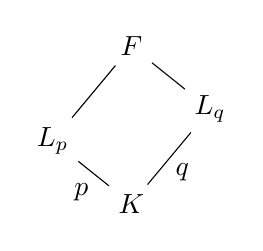
\begin{tikzpicture}

            \node (Q1) at (0,0) {$K$};
            \node (Q2) at (1,1.2) {$L_q$};
            \node (Q3) at (0,2) {$F$};
            \node (Q4) at (-1,0.8) {$L_p$};
        
            \draw (Q1)--(Q2) node [pos=0.8, below,inner sep=0.25cm] {$q$};
            \draw (Q1)--(Q4) node [pos=0.9, below,inner sep=0.25cm] {$p$};
            \draw (Q3)--(Q4);
            \draw (Q2)--(Q3);
        
        \end{tikzpicture}
        \caption[short]{Subfields of a $C_{pq}$-extension}
    \end{figure}
\end{proof}

We are finally ready to prove the main result of this section, from which Theorem \ref*{thm_consistent_cyclic} will follow. 

\begin{lemma}\label{lem_Cd_odd}
    Let $d$ be a composite, odd squarefree integer and let $F/K$ be a Galois extension of number fields such that $\Gal(F/K)=C_{d}$. Let $E/\QQ$ be an elliptic curve and let $L_k$ be the fields as above. Then
    $$\prod_{k\mid d}(C_{E/L_k})^{\mu(d/k)}$$
    is always a rational square.
\end{lemma}

\begin{proof}
    Let $n$ be the number of distinct prime numbers dividing $d$, so that $d=p_1\ldots p_n$ for some distinct odd primes $p_i$. We prove this result by induction. The base case for $n=2$ is the content of Lemma \ref*{lem_Cpq}. Assume that the result holds for squarefree integers with $n-1$ prime factors and consider the two sets of fields
    $$\mathcal{A}=\{L_k:p_n\nmid k\}\quad\text{and}\quad\mathcal{B}=\{L_k:p_n\mid k\},$$
    which are clearly a partition of all intermediate fields of $F/K$. Furthermore, the fields in $\mathcal{A}$ are precisely the intermediate fields of $K$ and $L_{d/p_n}$, while the fields in $\mathcal{B}$ are the intermediate fields of $L_{p_n}$ and $F$. However, since $\Gal(L_{d/p_n}/K)=\Gal(F/L_{p_n})=C_{d/p_n}$, it follows from the inductive hypothesis applied to the fields of $\mathcal{A}$ and $\mathcal{B}$ respectively that
    $$\prod_{k\mid \frac{d}{p_n}}(C_{E/L_k})^{\mu\left(\frac{d}{kp_n}\right)}\quad\text{and}\quad\prod_{p_n\mid k\mid d}(C_{E/L_{k}})^{\mu\left(d/k\right)}$$
    are both rational squares. By the natural decomposition
    $$\prod_{k\mid d}(C_{E/L_k})^{\mu(d/K)}=\prod_{k\mid \frac{d}{p_n}}(C_{E/L_k})^{\mu\left(d/k\right)}\prod_{p_n\mid k\mid d}(C_{E/L_{k}})^{\mu\left(d/k\right)}=\left(\prod_{k\mid \frac{d}{p_n}}(C_{E/L_k})^{\mu\left(\frac{d}{kp_n}\right)}\right)^{-1}\prod_{p_n\mid k\mid d}(C_{E/L_{k}})^{\mu\left(d/k\right)},$$
    it follows that the left hand side is also a rational square, as desired.
    \begin{figure}[!ht]
        \centering
        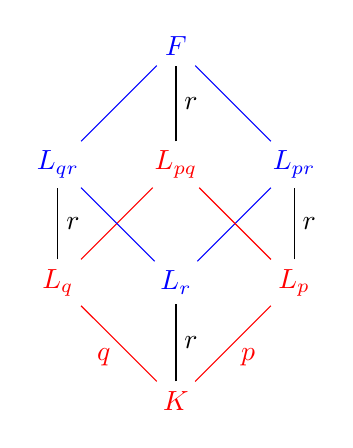
\begin{tikzpicture}

            \node [red] (Q1) at (0,0) {$K$};
            \node [red] (Q2) at (-1.5,1.5) {$L_q$};
            \node [blue] (Q3) at (0,1.5) {$L_r$};
            \node [red] (Q4) at (1.5,1.5) {$L_p$};
            \node [blue] (Q5) at (-1.5,3) {$L_{qr}$};
            \node [red] (Q6) at (0,3) {$L_{pq}$};
            \node [blue] (Q7) at (1.5,3) {$L_{pr}$};
            \node [blue] (Q8) at (0,4.5) {$F$};

            \draw [red] (Q1)--(Q2) node [pos=0.7, below,inner sep=0.25cm] {$q$};
            \draw [red] (Q1)--(Q4) node [pos=0.7, below,inner sep=0.25cm] {$p$};
            \draw (Q1)--(Q3) node [pos=0.5, right,inner sep=0.1cm] {$r$};
            \draw (Q2)--(Q5) node [pos=0.5, right,inner sep=0.1cm] {$r$};
            \draw (Q2)--(Q6) [red];
            \draw (Q3)--(Q5) [blue];
            \draw (Q3)--(Q7) [blue];
            \draw (Q4)--(Q6) [red];
            \draw (Q4)--(Q7) node [pos=0.5, right,inner sep=0.1cm] {$r$};
            \draw (Q5)--(Q8) [blue];
            \draw (Q6)--(Q8) node [pos=0.5, right,inner sep=0.1cm] {$r$};
            \draw (Q7)--(Q8) [blue];
        
        \end{tikzpicture}
        \caption[short]{Partition of $n=3$ into $n=2$. Red fields are in $\mathcal{A}$ while blue fields are in $\mathcal{B}$.}
    \end{figure}
\end{proof}

We are now ready to prove Theorem \ref*{thm_consistent_cyclic} for odd $d$.

\begin{proof}[Theorem \ref*{thm_consistent_cyclic} for odd $d$]
    The proof is divided into two cases depending on whether $d$ is the power of a prime or not. Suppose first that $d$ is not, so that $\rad(d)$ is a squarefree \textbf{composite} number. However, by Remark \ref*{rem_radical} and Lemma \ref*{lem_Cd_odd} we know that 
    $$\frac{\prod_i C_{E/F_i}}{\prod_j C_{E/F'_j}}$$
    is a rational square, and therefore it is the norm of an element for any quadratic extension of $\QQ$. 

    The case when $d=p^n$ for some odd prime $p$ and $n\geq1$ requires some more work. Lemma \ref*{lem_cyclic_decomp} and Lemma \ref*{lem_Cp} show that 
    $$\frac{\prod_i C_{E/F_i}}{\prod_j C_{E/F'_j}}=\frac{C_{E/F}}{C_{E/L_{p^{n-1}}}}$$
    is a rational square up to factors of $p$. Therefore, it suffices to show that $p$ is the norm of any quadratic subextension of $\QQ(\zeta_{p^n})$. Since $\Gal(\QQ(\zeta_{p^n})/\QQ)=(\ZZ/p^n\ZZ)$ is cyclic, $\QQ(\zeta_{p^n})$ has one unique quadratic subextension. Hence, it suffices to find the unique quadratic subextension of $\QQ(\zeta_p)$. A simple calculation shows that 
    $$\left(\sum_{a=0}^{p-1}\left(\frac{a}{p}\right)\zeta_p^a\right)^2=(-1)^{(p-1)/2}p,$$
    and therefore $\QQ(\sqrt{p^*})$ is the unique quadratic subextension of $\QQ(\zeta_p)$, where $p^*=(-1)^{(p-1)/2}p$. The fact that $p$ is a norm in this field is precisely the content of Corollary \ref*{p-norm}, and so the Theorem follows.
\end{proof}
 
\subsection*{Even Cyclic Extensions}
A bit more care is required to prove Theorem \ref*{thm_consistent_cyclic} for even $d$. This difficulty mainly lies in the case when $d$ is only divisible by one odd prime $p$. Likewise to the earlier case, we first prove some relevant results.

\begin{lemma}\label{lem_C2p}
    Let $p$ be an odd prime and let $F/K$ be a Galois extension of number fields such that $\Gal(F/K)=C_{2p}$ and let $L_k$ be the fields as above. Let $E/\QQ$ be an elliptic curve. Then
    $$\frac{C_{E/F}C_{E/K}}{C_{E/L_2}C_{E/L_p}}$$
    is a rational square up to factors of $p$.
\end{lemma}

\begin{proof}
    The proof is identical to the proof of Lemmas \ref*{lem_Cp} and \ref*{lem_Cpq} since the splitting behaviour of a prime $\pp$ in $K$ is again determined by $e_\pp$ and $f_\pp$. The following table records the contribution.

    \begin{table}[!ht]
        \centering
        \begin{tabular}{|l|l|l|l|l|l|l|}
        \hline
        $e_\pp$ & $f_\pp$  & $C_{\mathfrak{P}\mid \pp}(\QQ)$ & $C_{\mathfrak{P}\mid \pp}(L_p)$ & $C_{\mathfrak{P}\mid \pp}(L_2)$ & $C_{\mathfrak{P}\mid \pp}(F)$ & $\contr_\chi(\pp)$ \\ \hline
        $1$ & $1$ & $n;\tilde{n}$ & $n^p;\tilde{n}^p$ & $n^2;\tilde{n}^2$ & $n^{2p};\tilde{n}^{2p}$ & $\square$ \\ \hline
        $1$ & $p$ & $n;\tilde{n}$ & $n;\tilde{n}$ & $n^2;\tilde{n}^2$ & $n^2;\tilde{n}^2$ & $\square$ \\ \hline
        $1$ & $2$ & $n;\tilde{n}$ & $n^p;\tilde{n}^p$ & $n;n$ & $n^p;n^p$ & $\square$ \\ \hline
        $1$ & $2p$ & $n;\tilde{n}$ & $n;\tilde{n}$ & $n;n$ & $n;n$ & $\square$ \\ \hline
        $p$ & $1$ & $n;\tilde{n}$ & $pn;\tilde{n}$ & $n^2;\tilde{n}^2$ & $p^2n^2;\tilde{n}^2$ & $p\square;\square$ \\ \hline
        $p$ & $2$ & $n;\tilde{n}$ & $pn;\tilde{n}$ & $n;n$ & $pn;n$ & $\square$ \\ \hline
        $2$ & $1$ & $n;\tilde{n}$ & $n^p;\tilde{n}^p$ & $2n;1$ & $2^pn^p;1^p$ & $\square$ \\ \hline
        $2$ & $p$ & $n;\tilde{n}$ & $n;\tilde{n}$ & $2n;1$ & $2n;1$ & $\square$ \\ \hline
        $2p$ & $1$ & $n;\tilde{n}$ & $pn;\tilde{n}$ & $2n;1$ & $2pn;1$ & $\square$ \\ \hline
        \end{tabular}
    \end{table}
    The result follows again from \eqref{eqn_local_contr}.

\end{proof}

However, as soon as $d$ is divisible by $4$, the product of local factors is a rational square even if the individual contributions might not be, as the next lemma suggests. 

\begin{lemma}\label{lem_C4p}
    Let $p$ be an odd prime and let $F/K$ be a Galois extension of number fields such that $\Gal(F/K)=C_{4p}$ and let $L_k$ be the fields as above. Let $E/\QQ$ be an elliptic curve. Then
    $$\frac{C_{E/F}C_{E/L_2}}{C_{E/L_4}C_{E/L_{2p}}}$$
    is a rational square.
\end{lemma}

\begin{proof}
    All fields appearing in the product are intermediate fields of $L_2$ and $F$, and $\Gal(F/L_2)=C_{2p}$. Lemma \ref*{lem_C2p} shows that given some prime $\pp$ in $L_2$, $\contr_\chi(\pp)$ is a square unless $e_\pp=p$ and $f_\pp=1$. That is, $\pp$ ramifies in $L_{2p}/L_2$ and is split in $L_4/L_2$. Now consider $\bar\pp=\pp\cap\mathcal{O}_K$. Since $\pp$ splits in $L_4$, this forces $\bar{\pp}$ to split as well in $L_2/K$. Hence, $\bar{\pp}=\pp\pp'$ for two \textbf{distinct} primes in $K$ that have the same splitting behaviour and therefore $\contr_\chi(\pp)\contr_\chi(\pp')$ is a rational square, as desired.

    \begin{figure}[!ht]
        \centering
        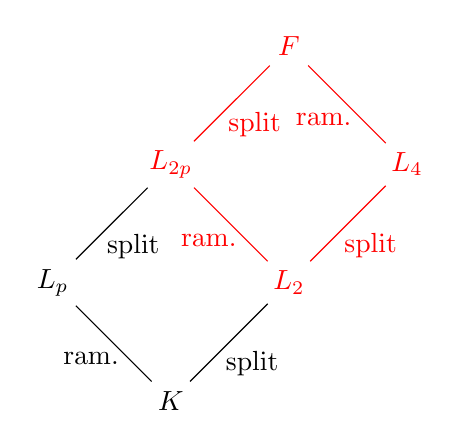
\begin{tikzpicture}

            \node (Q1) at (0,0) {$K$};
            \node (Q2) at (-1.5,1.5) {$L_p$};
            \node [red] (Q3) at (3,3) {$L_4$};
            \node [red] (Q4) at (1.5,1.5) {$L_2$};
            \node [red] (Q5) at (1.5,4.5) {$F$};
            \node [red] (Q6) at (0,3) {$L_{2p}$};
            

            \draw (Q1)--(Q2) node [pos=0.8, below,inner sep=0.4cm] {ram.};
            \draw (Q1)--(Q4) node [pos=0.8, below,inner sep=0.4cm] {split};
            \draw (Q2)--(Q6) node [pos=0.8, below,inner sep=0.4cm] {split};
            \draw [red] (Q3)--(Q5) node [pos=0.8, below,inner sep=0.4cm] {ram.};
            \draw [red] (Q4)--(Q6) node [pos=0.8, below,inner sep=0.4cm] {ram.};
            \draw [red] (Q6)--(Q5) node [pos=0.8, below,inner sep=0.4cm] {split};
            \draw [red] (Q4)--(Q3) node [pos=0.8, below,inner sep=0.4cm] {split};
        \end{tikzpicture}
        \caption[short]{\centering Field diagram for a $C_{4p}$ extension, together with the splitting\\ behaviour of a prime $\pp$ in $L_2$ with $e_\pp=p$ and $f_\pp=1$ over $F$.}
    \end{figure}
\end{proof}

We are now ready to prove Theorem \ref*{thm_consistent_cyclic} for even $d$. We break down the proof into three cases:

\subsubsection*{Case 1: $d$ is not divisible by any odd prime, so $d=2^l$}
If $l=1$, then $\QQ(\zeta_2)=\QQ$, so there is nothing to prove, so assume that $l\geq2$. If $\Gal(F/\QQ)=C_{2^l}$, then 
$$\frac{\prod_i C_{E/F_i}}{\prod_j C_{E/F'_j}}=\frac{C_{E/F}}{C_{E/L_{2^{l-1}}}},$$
and by Lemma \ref*{lem_Cp}, we know that this is a rational square up to factors of $2$, so it suffices to show that $2$ is a norm of every quadratic subfield of $\QQ(\zeta_{2^l})$. A standard argument shows that $\Gal(\QQ(2^l)/\QQ)=(\ZZ/2^l\ZZ)^*=C_{2^{l-2}}\times C_2$ and therefore $\QQ(\zeta_{2^l})$ has $\QQ(i)$ as its unique quadratic subextension if $l=2$ and has three quadratic subextensions if $l\geq 3$. Note that $\zeta_8=(1+i)/\sqrt{2}$ and therefore $\QQ(\zeta_8)=\QQ(i,\sqrt{2})$. The three quadratic subextensions are therefore $\QQ(i), \QQ(\sqrt{2})$ and $\QQ(\sqrt{-2})$. Then the result follows from the fact that 
$$2=\Norm_{\QQ(i)}(1+i)=\Norm_{\QQ(\sqrt{-2})}(2)=\Norm_{\QQ(\sqrt{2})}(2+\sqrt{2}).$$

\subsubsection*{Case 1: $d$ is divisible by at least two odd primes}
Let $K=L_{d/\rad(d)}$ be as in Remark \ref*{rem_radical} such that $\Gal(F/K)=C_{\rad(d)}$ and all fields appearing in the product of local factors contain $K$. Then using the same idea as in Lemma \ref*{lem_Cd_odd}, let 
$$\mathcal{A}=\{L_k\supseteq K:2\nmid [L_k:K]\}\quad\text{and}\quad\mathcal{B}=\{L_k\supseteq K:2\mid [L_k:K]\}.$$
Then the fiels in $\mathcal{A}$ and $\mathcal{B}$ are the intermediate fields of (distinct!) $C_{\rad(d)/2}$ extensions. These are odd cyclic extensions, and therefore by Lemma \ref*{lem_Cd_odd} the contribution is a rational square and therefore the norm of any quadratic extension.

\subsubsection*{Case 3: $d$ is divisible by one odd prime}
In this case, write $d=2^lp^n$ and let $L_k$ be the fields as above. In this case, we note that 
$$\frac{\prod_i C_{E/F_i}}{\prod_j C_{E/F'_j}}=\frac{C_{E/F}C_{E/L_{d/2p}}}{C_{E/L_{d/2}}C_{E/L_{d/p}}}.$$
By Lemma \ref*{lem_Cp}, we know that this product is a square up to multiples of $p$. If $l=1$, then $\Gal(\QQ(\zeta_{2p^n})/\QQ)=(\ZZ/2p^n\ZZ)^*=(\ZZ/p^n\ZZ)^*$ is cyclic, and therefore the unique quadratic subfield is $\QQ(\sqrt{p^*})$, and we already know that $p$ is a norm of this field.

From Lemma \ref*{lem_C2p} that the contribution of $p$ comes from those primes $\pp$ in $L_{d/2p}$ such that they ramify in $L_{d/2}$ and they split in $L_{d/p}$. However, as in the proof of Lemma \ref*{lem_C4p}, the prime $\bar{\pp}=\pp\cap L_{d/4p}$ must also split in $L_{d/2p}$ so $\bar{\pp}=\pp\pp'$ for $\pp'\neq\pp$ in $L_{d/2p}$. Since $\pp$ and $\pp'$ have the same splitting behaviour, they give the same contribution. Hence, the product of local terms is in fact a rational square and therefore the norm of any quadratic extension.

This concludes the proof of Theorem \ref*{thm_consistent_cyclic}, and we have in addition shown that the contribution is always a square except when $d=2^n,p^n$ or $2p^n$, where $p$ is an odd rational prime.
\qed

\subsection{Abelian Extensions}

\subsection{Odd-Degree Extensions}

\begin{appendices}
\section{Algebraic number theory background}
\subsection{Decompositions of primes in field extensions}
\subsection{Class field theory and genus fields}

In this section we introduce the concept of a genus field, as well as properties that will be useful for us.

Let $K$ be a number field. The \textbf{ideal class group} $\Cl_K = I_K / P_K$ is the group of fractional ideals modulo principal fractional ideals.
For an ideal $\fp$, we let $[\fp]$ denote its class in $\Cl_K$.

The \textbf{extended ideal class group} is the group $\Cl_K^{+} = I_K / P_K^{+}$, where
$P_K^{+}$ denotes the subgroup of principal fractional ideals with totally positive generator, i.e. ideals $\alpha \cO_K$ where $\sigma(\alpha) > 0$ for all real embeddings $\sigma \colon K \emb \bR$.

Note that $\Cl_K^{+}$ is the ray class group for the modulus $\fm$ of $K$ consisting of the product of all real places. The corresponding ray class field is known as the \textbf{extended Hilbert class field}, which we'll denote as $H^{+}$. This is the maximal extension of $K$ that is unramified at all finite primes. Let $H$ be the usual Hilbert Class field of $K$. Then one has $H \subset H^{+}$. Moreover, the index can be described in terms of the structure of $K$:

\begin{thm}\cite[Chapter VI, Section 3, Theorem 3.1]{Janusz}
    Let $r$ be the number of real primes of $K$. Let $U_K$, $U_K^{+}$ the group of units and totally positive units of $K$ respectively, Then 
    \[ [H^{+} \colon H] = 2^r [U_K \colon U_K^{+}]^{-1} .\]
\end{thm}
Observe that if $K$ has no real places, then $H^{+} = H$. For quadratic fields, the index depends on the norm of a fundamental unit:

\begin{cor}
    Let $K = \bQ(\sqrt{D})$ with $D$ a square-free positive integer. Let $\epsilon$ be a fundamental unit of $K$. Then $[H^{+} \colon H] = 1$ or $2$, according as $N_{K / \bQ}\left(\epsilon\right) = -1$ or $1$. 
\end{cor}


Fix $K = \bQ(\sqrt{D})$ for $D$ a squarefree integer. The (extended) Hilbert class field of $K$ need not be abelian over $\bQ$ (note that it is Galois over $\bQ$ by uniqueness of the (extended) Hilbert class field). However it can be useful to consider the maximal subfield of $H$ that is abelian over $\bQ$. 

\begin{defn}
    For any abelian extension $K / \bQ$, the \textbf{genus field} of $K / \bQ$ is the largest abelian extension $L / \bQ$ contained in $H$. The \textbf{extended genus field } is the largest abelian extension $L^{+} / \bQ $ contained in $H^{+}$.
\end{defn}

Let $\sigma \in \Gal(H^{+} / \bQ)$ be such that $\sigma|_{K}$ generates $\Gal(K / \bQ)$. $L$ has the following properties:

\begin{thm}\cite[Ch. VI, $\S$3, Theorem 3.3]{Janusz}\label{janusz-3.3}
    Let $K = \bQ(\sqrt{D})$.
    \begin{enumerate}
        \item $\Gal(H / L)$ is isomorphic to the subgroup of $C_K$ generated by the ideal classes of the form $[\sigma(\fU)\fU^{-1}]$, $\fU \in I_K$. 
        \item $\Gal(H / L) \simeq (C_K)^2$. 
    \end{enumerate}
\end{thm}

\begin{proof}[Proof sketch of 1.]
    Let $G = \Gal(H / \bQ)$. Then $L = H^{[G, G]}$ is the fixed field of the commutator subgroup of $G$. The Artin map induces an isomorphism $\varphi \colon C_K \to C \subset G$ with $\varphi(C_K) \simeq C = \Gal(H / K)$. One shows that $\varphi([\sigma(\fU)\fU^{-1}]) \in [G, C]$ and conversely that every commutator element in $[G, G]$ can be expressed as $\varphi([\sigma(\fU)\fU^{-1}])$ for some $\fU \in I_K$. 
\end{proof}

Note that this says that every class $[\sigma(\fU) \fU^{-1}]$ is a square in $C_K$.
This allows us to deduce the following:

\begin{thm}\label{p-principal}
Let $p$ be a prime in $\bQ$. If the residue degree of $p$ in $L / \bQ$ is $1$, then $p$ is the norm of a principal fractional ideal in $K$. 
\end{thm} 

\begin{proof}
Let $\varphi \colon C_K \to \Gal(H / K)$ be the isomorphism induced by the Artin map. By Theorem \ref{janusz-3.3}, $\Gal(L / K) = \Cl_K / \left(\Cl_K\right)^2$ is abelian. Let $\fp$ be a prime of $K$ lying over $p$. Then $N_{K / \bQ}(\fp) = p$ and $\fp$ has residue degree $1$ in $L$. It follows that $\varphi([\fp])|_{L} = \Id$ so that $\varphi([\fp]) \in \Gal(H / L)$. Thus by Theorem \ref{janusz-3.3} there is a fractional ideal $\fU$ of $I_K$ such that 
$[\fp] = [\sigma(\fU)\fU^{-1}]$. Observe that $N_{K / \bQ}(\sigma(\fU)\fU^{-1}) = 1$. It follows that we can represent $[\fp]^n$ by a fractional ideal of norm $p$ for all $n$. Since $\Cl_K$ is finite, this implies there is a principal fractional ideal in $K$ of norm $p$. 
\end{proof}

Observe that $C_K / (C_K)^2$ is an abelian group of exponent $2$. The following theorem describes its order:

\begin{thm} 
Suppose the discriminant of $K / \bQ$ has $t$ prime divisors. Then $C_K / (C_K)^2$ has order $2^{t-1}$ if $D < 0$ or if $D > 0$ and a unit of $K$ has norm $-1$. Otherwise, if $D > 0$ and all units of $K$ have norm $1$, it has order $2^{t - 2}$.
\end{thm} 

Our introduction of the extended genus field $L^{+}$ is mostly because it is easier to describe than $L$ when $K = \bQ(\sqrt{D})$.

\begin{thm} 
Let the discriminant of $K$ be $\Delta$ and suppose $|\Delta| = p_1 p_2 \cdots p_t$ where $p_2, \ldots p_t$ are odd primes, and $p_1$ is either odd or a power of $2$. Then the extended genus field of $K$ is 
    \[ L^{+} = \bQ(\sqrt{D}, \sqrt{p_2^*}, \ldots \sqrt{p_t^*}) = K(\sqrt{p_2^*}, \ldots \sqrt{p_t^*}), \] 
where 
\[ \begin{cases}
    p_i^* = p_i & \mathrm{if }\ p_i \equiv 1 \pmod 4, \\
    p_i^* = -p_i & \mathrm{if }\ p_i \equiv 3 \pmod 4
\end{cases}\]
\end{thm} 

\vspace{2em}

The following results are used in the body of the report:

\begin{cor}\label{p-one-mod-disc}
    Let $p$ be a prime in $\bQ$, $K = \bQ(\sqrt{D})$ with discriminant $\Delta$ such that $|\Delta| = p_1 p_2 \cdots p_t$, where all $p_i$ are odd primes. If $p \equiv 1 \mod {|\Delta|}$, then $p$ is the norm of a principal fractional ideal in $K$. It is also the norm of a principal fractional ideal in $K' = \bQ({\sqrt{p^*D}})$.
\end{cor}

\begin{proof}
    Any prime above $p$ in $K$ splits in $L^{+}$, hence also in $L$ (in particular it has residue degree $1$). Similarly for $K'$, the residue degree of $p$ in its extended genus field is $1$, and so in its genus field also. The result follows by Theorem \ref{p-principal}.
\end{proof}

We want to understand when $p$ is the norm of an element. Note that if $H = H^{+}$, then $p$ being the norm of a principal fractional ideal guarantees that it is the norm of an element. If $-1$ is a norm in our field then we are also fine. 

\begin{thm}\label{minus-one-norm}
Let $K = \bQ(\sqrt{D})$ with $D >0$ squarefree and suppose that all odd primes dividing $D$ are congruent to $1 \pmod 4$. Then $-1$ is the norm of an element of $K^{\times}$. 
\end{thm}

\begin{proof}
The condition on $D$ ensures that there exists $x$, $y \in \bQ$ such that $D = x^2 + y^2$. Therefore $-1 = (x / y)^2 - D(1/ y)^2$ so that $-1$ is the norm of the element $\frac{x}{y} + \frac{1}{y} \sqrt{D}$.

\end{proof}

Note that $-1$ being the norm of an element in $K$ does not ensure that $-1$ is the norm of a unit in $K$. The smallest counter-example is $K = \bQ(\sqrt{34})$. The element $\frac{5}{3} + \sqrt{34}$ has norm $-1$, but there is no unit with norm $-1$. 

\begin{thm}\label{p-norm-elem-1}
    Let $K = \bQ(\sqrt{D})$ and let $k$ be the minimal cyclotomic field such that $K \subset \bQ(\zeta_k)$. Suppose that $k$ is odd and $K$ is real.  If $p$ is a prime such that $p \equiv 1 \pmod {|\Delta|}$, then $p$ is the norm of an element from $K$. 
\end{thm}

\begin{proof}
    Note that $k$ being odd implies $D$ is odd. We know that $p$ is the norm of a principal fractional ideal of $K$ by corollary \ref{p-one-mod-disc}. Therefore there exists integers $x$, $y$, $z$ such that $\pm p z^2 = x^2 - Dy^2$. Suppose firstly that all primes dividing $D$ are congruent to $1 \pmod 4$. Then there is an element of $K^{\times}$ of norm $-1$ by Theorem \ref{minus-one-norm}. Hence we can find an element of norm $p$.

    Otherwise, there exists a prime $q \mid D$ such that $q \equiv 3 \pmod 4$. Reducing mod $q$, we have
    $ \pm p = \square$. Since $p \equiv 1 \pmod q$, it is a square $\pmod q$. But $-1$ is not a square mod $q$, hence our sign must have been $+$ and so $p$ is the norm of an element from $K^{\times}$.
\end{proof}

\begin{thm}\label{p-norm-elem-2}
    Let $K = \bQ(\sqrt{D})$ and let $k$ be the minimal cyclotomic field such that $K \subset \bQ(\zeta_k)$. Suppose that $k$ is odd and $K$ is real. Let $p$ be a prime such that $p \mid D$ and $p \equiv 1 \pmod q$ for all other primes $q \mid D$. Then $p$ is the norm of an element from $K$. 
\end{thm}

\begin{proof}
    By corollary \ref{p-one-mod-disc}, we know that $p$ is the norm of a principal fractional ideal of $K$. The rest of the argument is analogous to the previous proof.
\end{proof}


\begin{prop}
$\bQ(\sqrt{p^*})$ has odd narrow class number.
\end{prop}    

\begin{cor}\label{p-norm}
The prime $p \in \bQ$ is the norm of an element in $\bQ(\sqrt{p^*})^{\times}$.
\end{cor}

\begin{thm}\label{thm_class_number}
    Let $h(D)$ be the class number of $\QQ(\sqrt{D})$ and let $p$ be a rational prime. Then the following holds.
    \begin{itemize}
        \item If $p\equiv1\pmod{4}$, then $h(p)$ is odd and $h(-p)$ is even.
        \item If $p\equiv3\pmod{4}$, then $h(p)$ and $h(-p)$ are both odd.
    \end{itemize}
\end{thm}

\end{appendices}

\newpage

\bibliography{references.bib}
\bibliographystyle{amsalpha}


\end{document}